\setlength\abovedisplayskip{0pt} \setlength\belowdisplayskip{0pt}
\setlength\abovedisplayshortskip{0pt} \setlength\belowdisplayshortskip{0pt}

\chapter{Fundamentação Teórica} \label{cap:fundamentacao}
Neste capítulo serão abordados conceitos e explicações relacionadas aos tópicos apresentados neste trabalho, para proporcionar uma melhor compreensão sobre os mesmos.

\section{Distribuições Probabilísticas}

Ocorre frequentemente que, ao realizar uma experiência, tem-se interesse principalmente em algumas funções do resultado, em oposição ao resultado em si - por exemplo, ao jogar dados, muitas vezes o interesse se encontra na soma dos dois dados e não no resultado real, individual de cada dado \cite{ross}. Ou seja, pode-se querer saber que a soma é sete e não se preocupar se o resultado real foi (1, 6) ou (2, 5) ou (3, 4) ou (4, 3) ou (5, 2) ou (6, 1). Essas quantidades de interesse, ou mais formalmente, essas funções de valor real definidas no espaço de amostra são conhecidas como variáveis aleatórias \cite{ross}.

Existem dois tipos de variáveis aleatórias, variáveis aleatórias discretas e variáveis aleatórias contínuas: variáveis discretas podem assumir apenas um número contável de valores, enquanto variáveis contínuas (as que serão utilizadas neste trabalho) possuem um conjunto incontável de possíveis valores \cite{ross}.

Sendo $X$ uma variável aleatória; pode-se dizer que $X$ é uma variável contínua se existir uma função não-negativa $f(x)$, definida para todos os números reais $x \in (-\infty, \infty)$, de forma que para qualquer conjunto $B$ de números reais a seguinte propriedade é válida \cite{ross}:

\begin{equation}
\label{eq:1}
    P\{X \in B\} = \int_{B} f(x) dx
\end{equation}

A função $f(x)$ é chamada de função densidade da variável aleatória $X$ - em outras palavras, a equação \ref{eq:1} mostra que a probabilidade de $X$ estar no conjunto $B$ pode ser obtida integrando a função densidade sobre o conjunto $B$ \cite{ross}.

Variáveis aleatórias são tão importantes em experimentos aleatórios que às vezes o espaço amostral original do experimento é ignorado e foca-se na distribuição probabilística da variável aleatória \cite{montgomery}. A distribuição probabilística de uma variável aleatória $X$ é uma descrição das probabilidades
associadas a possíveis valores de $X$; e em alguns casos, é conveniente expressar a probabilidade em termos de uma fórmula \cite{montgomery}.

A seguir serão apresentadas algumas das distribuições probabilísticas mais conhecidas, para melhor compreensão.

\subsection{Distribuição Uniforme}
A distribuição Uniforme é um método de randomização que distribui uniformemente os valores em um intervalo formado por seus dois parâmetros: \textit{a}, o limite inferior; e \textit{b}, o limite superior - essa distribuição é caracterizada por possuir a mesma probabilidade para todos os sub-intervalos com mesmo tamanho, e sua função de densidade é a seguinte \cite{fister}:

\begin{equation}
P(x) = 
\begin{cases}
	\frac{1}{b - a}    & \text{$a \leq x \leq b$}\\
    0 & \text{caso contrário.}
\end{cases}
\end{equation}

Uma representação visual em 1D da distribuição Uniforme pode ser vista na figura \ref{fig:1DUniforme}, onde 2000 pontos foram randomicamente gerados utilizando a mesma. O gráfico é composto pelo eixo x, onde tem-se a quantidade de pontos gerados; e pelo eixo y, onde tem-se os respectivos números que foram gerados, em um intervalo de $[0, 100]$.

{
    \centering
    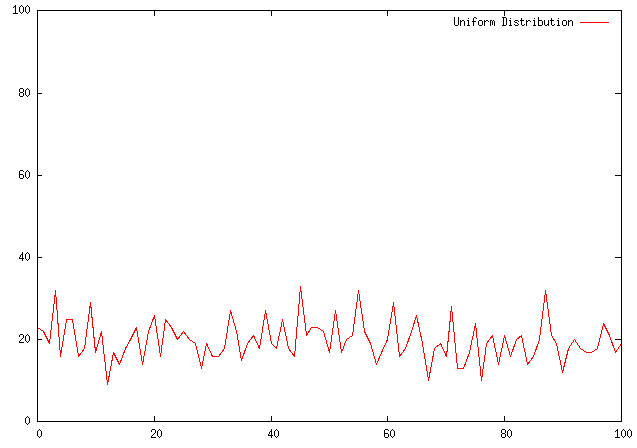
\includegraphics[width=0.5\linewidth]{figuras/DistribuicaoUniforme.png}
    \captionof{figure}{Representação Visual da Distribuição Uniforme}
    \label{fig:1DUniforme}
    \source{Própria autora.}
}

\subsection{Distribuição Gaussiana}
A distribuição Gaussiana ou Normal é definida por dois parâmetros: a média ($\mu$) e o desvio-padrão ($\sigma$) \cite{fister}. Essa distribuição tem uma propriedade, onde aproximadamente dois terços dos valores caem em até um desvio-padrão da média, e a sua função de densidade é apresentada em \ref{eq:2} \cite{fister}:

\begin{equation}
\label{eq:2}
P(x) = \frac{1}{\sigma \sqrt{2\pi}}e^{-\frac{1}{2}(\frac{x - \mu}{\sigma})^2}
\end{equation}

Uma representação visual em 1D da distribuição Gaussiana pode ser vista na figura \ref{fig:1DGaussiana}, onde 2000 pontos foram randomicamente gerados utilizando a mesma, com parâmetros $\mu = 50$ e $\sigma = 15$. O gráfico é composto pelo eixo x, onde tem-se a quantidade de pontos gerados com certo número; e pelo eixo y, onde tem-se os respectivos números que foram gerados, em um intervalo de $[0, 100]$.

{
    \centering
    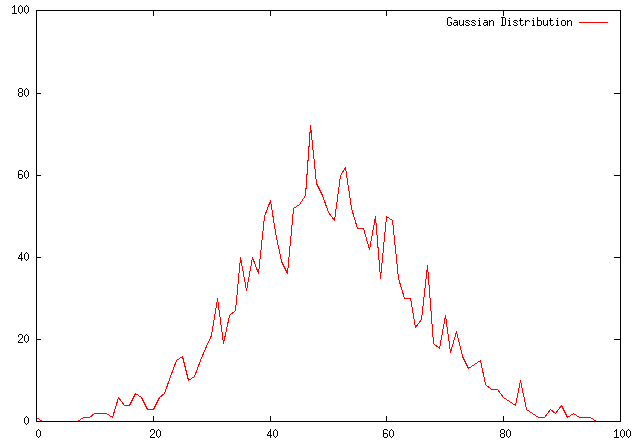
\includegraphics[width=0.5\linewidth]{figuras/DistribuicaoGaussiana.png}
    \captionof{figure}{Representação Visual da Distribuição Gaussiana}
    \label{fig:1DGaussiana}
    \source{Própria autora.}
}

\subsection{Distribuição de Cauchy}
A distribuição de Cauchy é também definida por dois parâmetros: $\alpha$ e $\beta$, parâmetros que afetam a média e a extensão da distribuição respectivamente, e sua função de densidade é como a seguir \cite{thomsen}:

\begin{equation}
P(x) = \frac{1}{\beta \pi (1 + (\frac{x - \alpha}{\beta})^2)}
\end{equation}

Uma representação visual em 1D da distribuição de Cauchy pode ser vista na figura \ref{fig:1DCauchy}, onde 2000 pontos foram randomicamente gerados utilizando a mesma, com parâmetros $\alpha = 50$ e $\beta = 10$. O gráfico é composto pelo eixo x, onde tem-se a quantidade de pontos gerados; e pelo eixo y, onde tem-se os respectivos números que foram gerados, em um intervalo de $[0, 100]$.

{
    \centering
    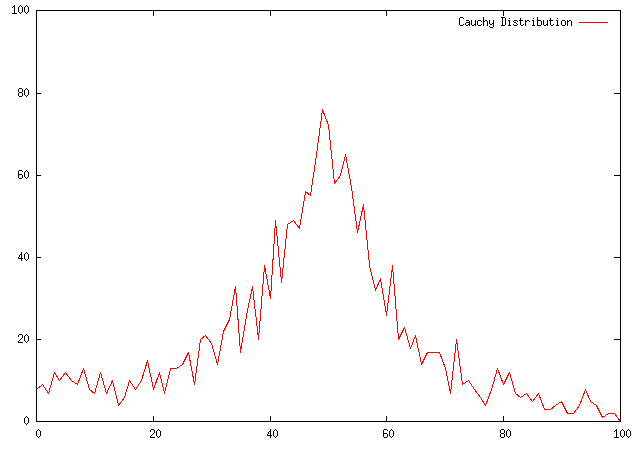
\includegraphics[width=0.5\linewidth]{figuras/DistribuicaoCauchy.png}
    \captionof{figure}{Representação Visual da Distribuição de Cauchy}
    \label{fig:1DCauchy}
    \source{Própria autora.}
}

\subsection{Distribuição Exponencial}

A distribuição Exponencial descreve o tempo entre eventos em um processo de Poisson e é definida por dois parâmetros: \textit{x0}, que define o ponto inicial da distribuição e $\gamma$, que define a inclinação da curva da função de densidade da probabilidade, que é definida pela fórmula \ref{eq:exponencial} \cite{yu} \footnote{O asterisco encontrado nessa e em algumas outras referências representa os artigos resultantes do mapeamento sistemático da literatura, apresentado mais a frente no trabalho.}.

\begin{equation}
\label{eq:exponencial}
P(x) = 
\begin{cases}
	\gamma e^{-\gamma(x-x0)},    & \text{$x \geq 0$}\\
    0, & \text{x < 0}
\end{cases}
\end{equation}

Uma representação visual em 1D da distribuição Exponencial pode ser vista na figura \ref{fig:1DExponencial}, onde 2000 pontos foram randomicamente gerados utilizando a mesma, com parâmetros $x0 = 0$ e $\gamma = 0,5$. O gráfico é composto pelo eixo x, onde tem-se a quantidade de pontos gerados; e pelo eixo y, onde tem-se os respectivos números que foram gerados, em um intervalo de $[0, 100]$.

{
    \centering
    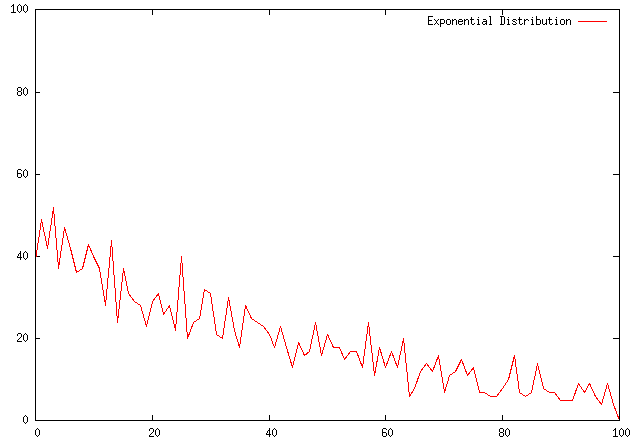
\includegraphics[width=0.5\linewidth]{figuras/DistribuicaoExponencial.png}
    \captionof{figure}{Representação Visual da Distribuição Exponencial}
    \label{fig:1DExponencial}
    \source{Própria autora.}
}

\subsection{Distribuição Rayleigh}

A distribuição de Rayleigh possui apenas um parâmetro: $\sigma$, que é responsável por controlar a planicidade da forma da função de densidade, que é definida pela equação \ref{eq:rayleigh} \cite{yu}.

\begin{equation}
\label{eq:rayleigh}
P(x) = \frac{x}{\sigma^{2}}e^{-\frac{x^{2}}{2\sigma^{2}}},  \text{x $\geq$ 0}
\end{equation}

Uma representação visual em 1D da distribuição Rayleigh pode ser vista na figura \ref{fig:1DRayleigh}, onde 2000 pontos foram randomicamente gerados utilizando a mesma, com parâmetro $\sigma = 0,2$. O gráfico é composto pelo eixo x, onde tem-se a quantidade de pontos gerados; e pelo eixo y, onde tem-se os respectivos números que foram gerados, em um intervalo de $[0, 100]$.

{
    \centering
    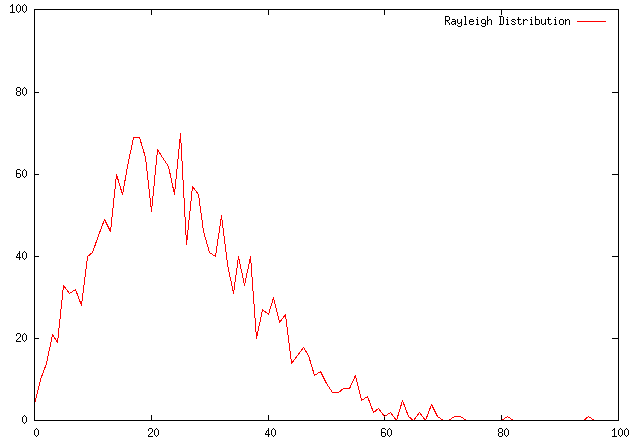
\includegraphics[width=0.5\linewidth]{figuras/DistribuicaoRayleigh.png}
    \captionof{figure}{Representação Visual da Distribuição Rayleigh}
    \label{fig:1DRayleigh}
    \source{Própria autora.}
}

\subsection{Distribuição Beta}

A distribuição Beta padrão possui dois parâmetros: a e b e sua função de densidade é dada pela equação \ref{eq:beta}, onde $\Gamma$ define a função Gamma \cite{ali}.

\begin{equation}
\label{eq:beta}
P(x) = \frac{\Gamma(a+b)}{\Gamma(a) + \Gamma(b)}x^{(a-1)}(1-x)^{(b-1)}, \text{ a, b > 0}
\end{equation}

Uma representação visual em 1D da distribuição Beta pode ser vista na figura \ref{fig:1DBeta}, onde 2000 pontos foram randomicamente gerados utilizando a mesma, com parâmetros $a = 2$ e $b = 2$. O gráfico é composto pelo eixo x, onde tem-se a quantidade de pontos gerados; e pelo eixo y, onde tem-se os respectivos números que foram gerados, em um intervalo de $[0, 100]$.

{
    \centering
    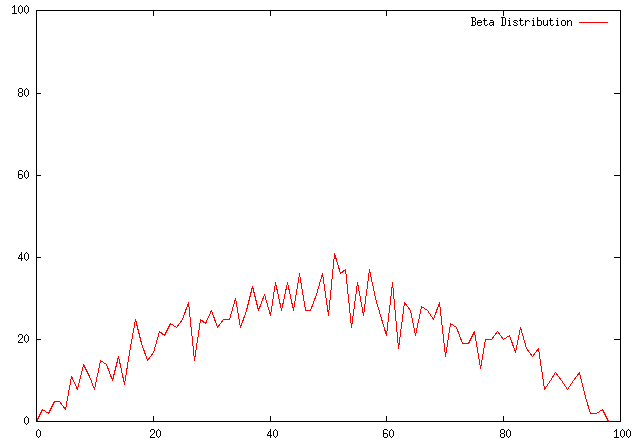
\includegraphics[width=0.5\linewidth]{figuras/DistribuicaoBeta.png}
    \captionof{figure}{Representação Visual da Distribuição Beta}
    \label{fig:1DBeta}
    \source{Própria autora.}
}

\section{Mapas Caóticos}

Um sistema dinâmico consiste em um conjunto de possíveis estados juntamente com uma regra que determina o estado atual em termos de estados passados - esta regra deve ser determinística, o que significa que pode-se determinar o estado atual unicamente a partir dos estados passados; além disso, nenhuma aleatoriedade é permitida nesta definição de sistemas dinâmicos determinísticos \cite{alligood}.

%Existem dois tipos de sistemas dinâmicos \cite{alligood}. Se a regra for aplicada em momentos discretos, chamamos o sistema de sistema dinâmico de tempo discreto \cite{alligood}. Um sistema de tempo discreto tem o estado atual como entrada e atualiza a situação através da produção de um novo estado como saída \cite{alligood}. Pelo estado do sistema, queremos dizer qualquer informação que é necessária para a regra ser aplicada \cite{alligood}.

%O outro tipo de sistema dinâmico é essencialmente o limite dos sistemas discretos com tempos de atualização menores \cite{alligood}. A regra que governa neste caso se torna um conjunto de equações diferenciais, e o termo sistemas dinâmicos de tempo contínuo é utilizado \cite{alligood}.

Existem sistemas dinâmicos determinísticos nos quais a evolução temporal tem uma dependência forte nas condições iniciais, ou seja, as equações diferenciais que governam a evolução do sistema são muito sensíveis às condições iniciais \cite{cattani}. Dessa maneira, medidas feitas em um estado do sistema em um certo momento podem não nos permitir prever a situação futura do sistema, apesar do fato de que as equações governantes são bem conhecidas \cite{cattani}, visto que esses sistemas se comportam de maneira imprevisível \cite{fister}. Por definição, essas equações são chamadas de caóticas.

Em alguns casos, é muito difícil estudar a evolução de um sistema integrando suas equações diferenciais, e às vezes também é difícil construir um modelo matemático exato para estudar o sistema - nesses casos, é possível conseguir uma boa descrição de um processo caótico usando um modelo iterativo algébrico chamado mapeamento \cite{cattani}.

Existem inúmeros sistemas caóticos que são estudados utilizando a abordagem de mapeamento \cite{cattani}. Algumas dessas abordagens são apresentadas a seguir.

\subsection{Mapa Logístico}
O mapa Logístico é um mapa caótico. É determinado pela equação \ref{eq:logistic} onde $x_{n} \in$ $[0, 1]$ e $r$ é um parâmetro que quando igual a 4 apresenta comportamento caótico \cite{fister}.

\begin{equation}
\label{eq:logistic}
x_{n + 1} = r x_{n} (1 - x_{n})
\end{equation}

Uma representação visual em 1D do mapa Logístico pode ser vista na figura \ref{fig:1DLogistico}, onde 2000 pontos foram randomicamente gerados utilizando a mesmo. O gráfico é composto pelo eixo x, onde tem-se a quantidade de pontos gerados; e pelo eixo y, onde tem-se os respectivos números que foram gerados, em um intervalo de $[0, 100]$.

{
    \centering
    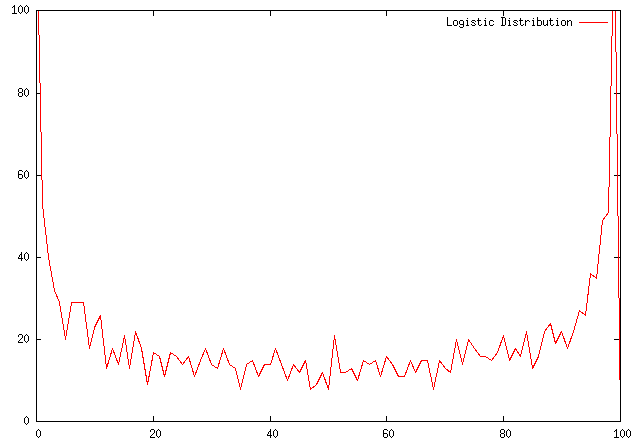
\includegraphics[width=0.55\linewidth]{figuras/DistribuicaoLogistica.png}
    \captionof{figure}{Representação Visual do Mapa Logístico}
    \label{fig:1DLogistico}
    \source{Própria autora.}
}

% \subsection{Mapa de Kent}
% Por fim, o mapa de Kent é também um mapa caótico, definido pela equação \ref{eq:kent}, onde $x(n) \in$ $[0, 1]$ e $m$ é um número no intervalo $0 < m < 1$ que quando igual a 0.3 apresenta comportamento caótico \cite{fister}. 

% \begin{equation}
% \label{eq:kent}
% x(n + 1) = 
% \begin{cases}
% 	\frac{x(n)}{m}    & \text{$0 < x(n) \leq m$}\\
%     \frac{1 - x(n)}{1 - m} & \text{$m < x(n) < 1$}
% \end{cases}
% \end{equation}

\subsection{Mapa Sinusoidal}

Esse mapa caótico pode ser definido pela fórmula \ref{eq:sinusoidal}, onde quando a = 2,3 ele exibe comportamento caótico \cite{gandomi}.

\begin{equation}
\label{eq:sinusoidal}
x_{n + 1} = a x_{n}^{2} sin(\pi x_{n})
\end{equation}

Uma representação visual em 1D do mapa Sinusoidal pode ser vista na figura \ref{fig:1DSinusoidal}, onde 2000 pontos foram randomicamente gerados utilizando a mesmo. O gráfico é composto pelo eixo x, onde tem-se a quantidade de pontos gerados; e pelo eixo y, onde tem-se os respectivos números que foram gerados, em um intervalo de $[0, 100]$.

{
    \centering
    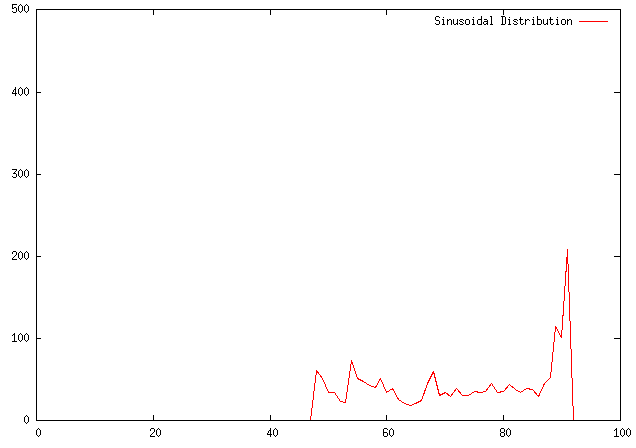
\includegraphics[width=0.55\linewidth]{figuras/DistribuicaoSinusoidal.png}
    \captionof{figure}{Representação Visual do Mapa Sinusoidal}
    \label{fig:1DSinusoidal}
    \source{Própria autora.}
}

\subsection{Mapa Piecewise}

O mapa caótico Piecewisse, é definido pela fórmula \ref{eq:piecewise}, onde P é o parâmetro de controle, normalmente escolhido entre 0,0 e 0,5 \cite{gandomi}.

\begin{equation}
\label{eq:piecewise}
x_{n + 1} =
\begin{cases}
    \frac{x_{n}}{P}, & \text{$0 \leq x_{n} < P$}\\
    \frac{x_{n} - P}{0,5 - P}, & \text{$P \leq x_{n} < \frac{1}{2}$}\\
    \frac{1-P-x_{n}}{0,5 - P}, & \text{$\frac{1}{2} \leq x_{n} < 1-P $}\\
    \frac{1-x_{n}}{P}, & \text{$1-P \leq x_{n} < 1$}\\
\end{cases}
\end{equation}

Uma representação visual em 1D do mapa Piecewise pode ser vista na figura \ref{fig:1DPiecewise}, onde 2000 pontos foram randomicamente gerados utilizando a mesmo. O gráfico é composto pelo eixo x, onde tem-se a quantidade de pontos gerados; e pelo eixo y, onde tem-se os respectivos números que foram gerados, em um intervalo de $[0, 100]$.

{
    \centering
    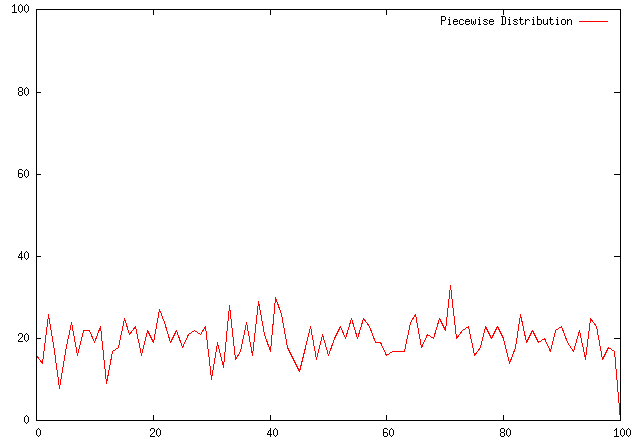
\includegraphics[width=0.55\linewidth]{figuras/DistribuicaoPiecewise.png}
    \captionof{figure}{Representação Visual do Mapa Piecewise}
    \label{fig:1DPiecewise}
    \source{Própria autora.}
}

\subsection{Mapa Tent}

O mapa caótico Tent é similar ao mapa Logístico e é definido pela equação \ref{eq:tent} \cite{gandomi}.

\begin{equation}
\label{eq:tent}
x_{n + 1} =
\begin{cases}
    \frac{x_{n}}{0,7}, & \text{$x_{n} < 0,7$} \\
    \frac{10}{3}(1-x_{n}) & \text{$x_{n} \geq 0,7$} 
\end{cases}
\end{equation}

Uma representação visual em 1D do mapa Tent pode ser vista na figura \ref{fig:1DTent}, onde 2000 pontos foram randomicamente gerados utilizando a mesmo. O gráfico é composto pelo eixo x, onde tem-se a quantidade de pontos gerados; e pelo eixo y, onde tem-se os respectivos números que foram gerados, em um intervalo de $[0, 100]$.

{
    \centering
    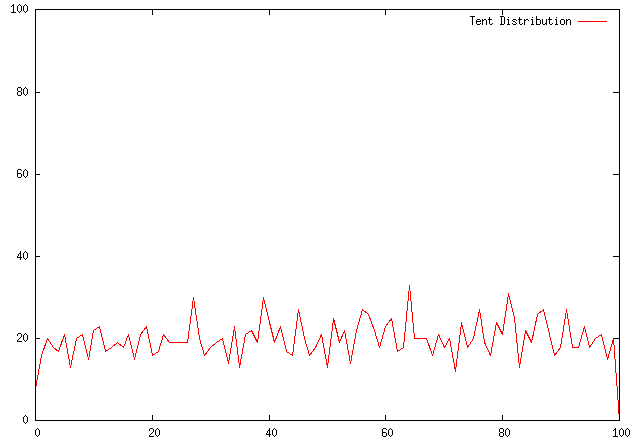
\includegraphics[width=0.55\linewidth]{figuras/DistribuicaoTent.png}
    \captionof{figure}{Representação Visual do Mapa Tent}
    \label{fig:1DTent}
    \source{Própria autora.}
}

\subsection{Mapa Circle}

O mapa Circle é representado pela equação \ref{eq:circle}, e quando seus parâmetros a e b forem igualados a 0,5 e 0,2, respectivamente, ele apresenta um comportamento caótico \cite{gandomi}.

\begin{equation}
\label{eq:circle}
x_{n + 1} = x_{n} + b - (\frac{a}{2\pi}) sin(2\pi x_{n})mod(1)
\end{equation}

Uma representação visual em 1D do mapa Circle pode ser vista na figura \ref{fig:1DCircle}, onde 2000 pontos foram randomicamente gerados utilizando a mesmo. O gráfico é composto pelo eixo x, onde tem-se a quantidade de pontos gerados; e pelo eixo y, onde tem-se os respectivos números que foram gerados, em um intervalo de $[0, 100]$.

{
    \centering
    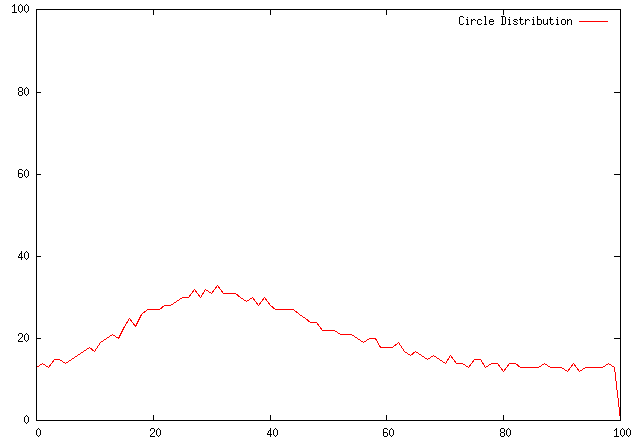
\includegraphics[width=0.55\linewidth]{figuras/DistribuicaoCircle.png}
    \captionof{figure}{Representação Visual do Mapa Circle}
    \label{fig:1DCircle}
    \source{Própria autora.}
}

% Para melhor visualização, a figura \ref{fig:dist} apresenta uma representação visual em 1D de como cada método distribui 2000 valores em um intervalo de $[0, 100]$. Em relação à aplicação em meta-heurísticas, podemos observar nos gráficos que a distribuição uniforme e o mapa caótico de Kent realizam uma diversificação do espaço de busca, distribuindo os valores de forma espaçada no intervalo. Já as distribuições Gaussiana ($\mu = 50$ e $\sigma = 15$), de Cauchy ($\alpha = 50$ e $\beta = 10$) e o mapa caótico Logístico apresentam uma intensificação do espaço de busca, focando a distribuição de valores em torno de um local específico do intervalo.

% {
%     \centering
%     \includegraphics[width=0.9\linewidth]{figuras/montagem1D.png}
%     \captionof{figure}{Representação visual em 1D das distribuições}
%     \label{fig:dist}
% }

\section{Meta-heurísticas}

% Na área de otimização, a classificação dos algoritmos pode ser dada através da sua natureza, dividindo os mesmos em duas categorias: algoritmos determinísticos e algoritmos estocásticos \cite{yang}. Algoritmos determinísticos seguem um procedimento rigoroso, e o caminho e valores de suas variáveis e função são repetíveis; por exemplo, o algoritmo subida de encosta é determinístico, pois a partir de um mesmo ponto de partida ele seguirá o mesmo caminho sempre \cite{yang}. Por outro lado, algoritmos estocásticos sempre terão algum tipo de aleatoriedade; algoritmos genéticos são um bom exemplo, onde o vetor de soluções será diferente a cada rodada, visto que o algoritmo utiliza um gerador de números pseudo-aleatórios \cite{yang}.

% Algoritmos estocásticos possuem dois tipos: heurísticas e meta-heurísticas \cite{yang}. Explicando de forma vaga, heurística significa "descobrir através de tentativa e erro" - soluções boas para um problema complexo podem ser encontradas em um tempo razoável, mas não existe garantia que a solução ótima será encontrada \cite{yang}. Mais adiante, foram desenvolvidas as meta-heurísticas, que significam "além" ou "alto-nível" e elas geralmente possuem um desempenho melhor do que as heurísticas \cite{yang}.

Como dito anteriormente, as meta-heurísticas são métodos que significam "além" \- ou "alto-nível" \- e possuem, geralmente, um desempenho melhor do que as heurísticas \cite{yang}. Além disso, todos os algoritmos meta-heurísticos usam uma combinação entre aleatoriedade/randomização e busca local \cite{yang}. As meta-heurísticas podem ser consideradas como uma maneira eficiente de produzir soluções aceitáveis através da tentativa e erro, para problemas complexos, em um tempo razoavelmente prático \cite{yang2}.

Em geral, o desempenho de meta-heurísticas depende de dois componentes chaves, intensificação e diversificação: intensificação significa focar a busca em uma região local explorando a informação de que uma solução ótima atual se encontra nessa região \cite{sahib}. A intensificação usa qualquer informação do problema de interesse para gerar novas soluções que são melhores do que as soluções encontradas anteriormente; a vantagem disso é que usualmente ela leva a níveis de convergência altos, e a desvantagem é que ela pode ficar facilmente presa em ótimos locais \cite{sahib}. 

Já a diversificação ajuda a gerar soluções diversas com o objetivo de explorar o espaço de busca em uma escala global, permitindo assim explorar esse espaço de uma forma mais eficiente, e gerar soluções distantes das soluções atuais; a vantagem disso é que ela é menos provável de ficar presa em ótimos locais, e a otimalidade global pode se tornar mais alcançável, entretanto, sua desvantagem é que pode levar à uma velocidade de convergência muito lenta \cite{sahib}.

O balanço entre esses dois componentes é extremamente importante para a eficiência e desempenho do algoritmo - muita intensificação e pouca diversificação pode causar o algoritmo a ficar preso em ótimos locais, o que pode dificultar ou até prevenir o algoritmo de encontrar o ótimo global \cite{yang2}. Por outro lado, muita diversificação e pouca intensificação pode dificultar o objetivo do algoritmo de convergir, diminuindo seu desempenho \cite{yang2}.

A seguir serão apresentadas e explicadas as meta-heurísticas que serão aplicadas neste trabalho.

\subsection{Evolução Diferencial}
\label{sub:de}

A Evolução Diferencial (DE) é um algoritmo evolucionário para otimização global sobre espaços contínuos \cite{brest}. De forma geral, o algoritmo cria novos candidatos à solução combinando o indivíduo parente e diversos outros indivíduos da mesma população \cite{brest}. O candidato apenas substitui o parente se possuir um valor \textit{fitness} melhor \cite{brest}. A Evolução Diferencial possui três parâmetros:

\begin{itemize}
    \item F: fator de amplificação do vetor de diferença (escala de mutação);
    \item CR: parâmetro de controle de \textit{crossover};
    \item NP: tamanho da população.
\end{itemize}

A população inicial é selecionada de forma randômica entre os limites inferior e superior \cite{brest}. Então a DE realiza um processo chamado evolução: para cada geração a DE emprega as operações de mutação e \textit{crossover} para produzir um vetor \textit{trial} \cite{brest}. Logo após, a operação de seleção é utilizada para escolher os vetores para a próxima geração \cite{brest}. 

\subsubsection{Mutação}

A mutação cria um vetor mutante para cada vetor da população. Eles podem ser criados usando uma estratégia de mutação, como por exemplo: rand/1; best/1; current to best/1; best/2; rand/2; entre outras \cite{brest}. A estratégia de mutação utilizada neste trabalho é a rand/1, que é dada pela seguinte fórmula \cite{brest}:

\begin{equation}
v_{i,G} =  x_{r1,G} + F * (x_{r2,G} - x_{r3,G}) 
\end{equation}

Onde os índices r1, r2 e r3 representam valores inteiros randômicos, divergentes uns dos outros e do índice i, gerados no intervalo $[1, NP]$. \cite{brest}.

\subsubsection{Crossover}

Depois da mutação, uma operação de \textit{crossover} binária é realizada para formar o vetor \textit{trial} final, de acordo com o vetor $i$ da população e seu vetor mutante correspondente \cite{brest}. A fórmula utilizada é a seguinte \cite{brest}:

\begin{equation}
u_i,_j,_G = 
\begin{cases}
	V_{i,j,G}    & \text{se $rand(0, 1) \leq CR$ or $j = j_{rand}$}\\
    x_{i,j,G} & \text{caso contrário.}
\end{cases}
\end{equation}

Onde $x$ é o vetor da população; $v$ é o vetor mutante; $i$ é o índice no intervalo $[1, NP]$; $j$ é o índice no intervalo $[1, D]$ sendo D a quantidade de dimensões do problema; e $j_{rand}$ é um índice escolhido de forma aleatória dentro do intervalo $[1, NP]$. 

\subsubsection{Seleção}

A seleção seleciona, de acordo com o valor \textit{fitness} do vetor da população e do seu vetor \textit{trial} correspondente, qual vetor irá sobreviver e se tornar um membro da próxima geração \cite{brest}.

\subsubsection{Evolução Diferencial Auto-Adaptativa}

A Evolução Diferencial Auto-Adaptativa (jDE) usa um mecanismo auto-adaptativo para controlar os parâmetros F e CR \cite{brest}. Cada indivíduo da população é estendido para possuir seus próprios valores de F e CR \cite{brest}. Melhores valores para esses parâmetros de controle levam a melhores indivíduos, que consequentemente, possuem mais chances de sobreviver e produzir descendentes, propagando esses melhores valores de parâmetros \cite{brest}.

Então, os valores para os parâmetros de controle são calculados como a seguir \cite{brest}:

\begin{equation}
F_{i,G+1} = 
\begin{cases}
	Fl + rand1 * Fu    & \text{se $rand2 < T1$}\\
    F_{i,G} & \text{caso contrário.}
\end{cases}
\end{equation}

\begin{equation}
CR_{i,G+1} = 
\begin{cases}
	rand3    & \text{se $rand4 < T2$}\\
    CR_{i,G} & \text{caso contrário.}
\end{cases}
\end{equation}

Onde $randj, j \in \{1, 2, 3, 4\}$ são valores uniformemente distribuídos em um intervalo de $[0, 1]$; e F1, Fu, T1 e T2 são valores fixos com os respectivos números: 0,1, 0,9, 0,1 e 0,1 \cite{brest}.

Como pode-se observar no diagrama da figura \ref{fig:jDE}, tem-se que o algoritmo utiliza a randomização em cinco partes do seu processo e estão anotados em caixas cinzas no diagrama: ao inicializar os agentes no espaço de busca; ao calcular os novos parâmetros F e CR; ao realizar a operação de mutação e por fim, ao realizar a operação de \textit{crossover}. O jDE utiliza, por padrão, a distribuição uniforme para realizar todas essas randomizações.

{
    \centering
    \centerline{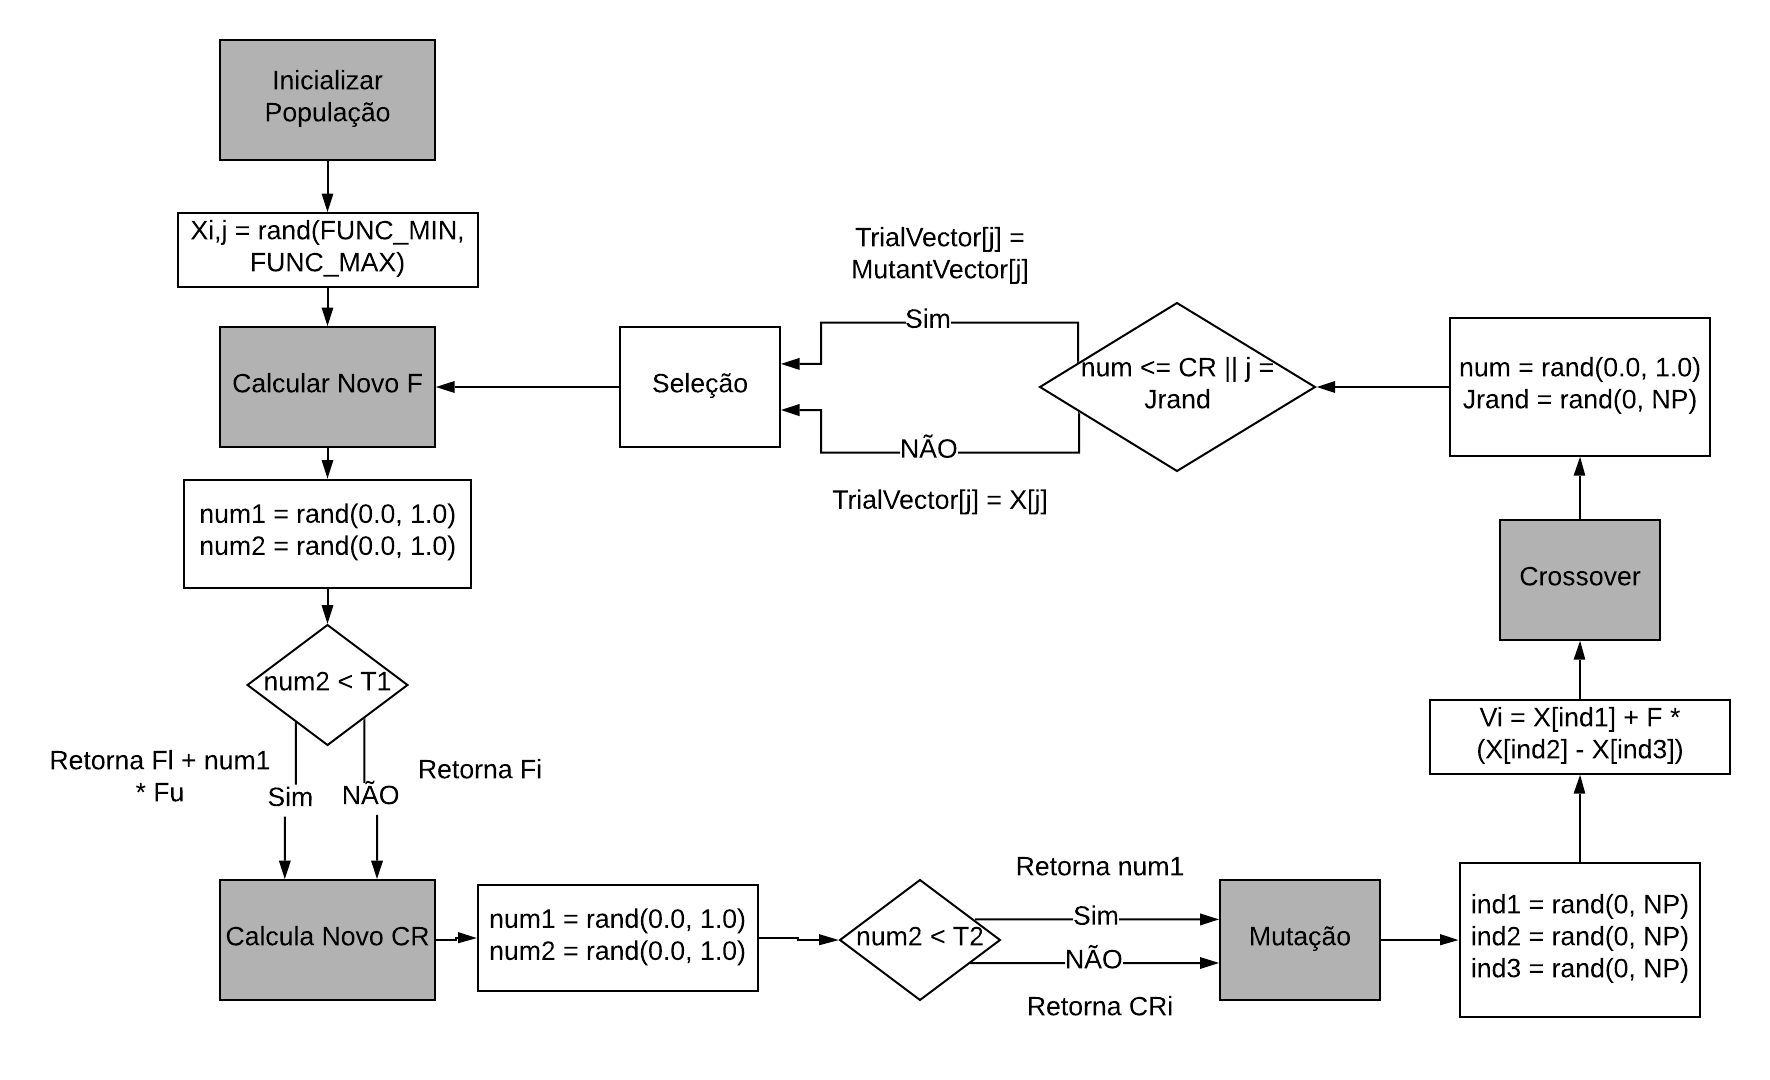
\includegraphics[width=1.1\linewidth]{figuras/Diagrama_de_Blocos.png}}
    \captionof{figure}{Diagrama de Blocos do jDE}
    \label{fig:jDE}
    \source{Própria autora.}
}

\subsection{Algoritmo Seno e Cosseno}
\label{sub:sca}

O SCA (\textit{Sine Cosine Algorithm}) cria múltiplas soluções randômicas iniciais e requer que as mesmas flutuem em direção ou na direção oposta da melhor solução usando um modelo matemático baseado nas funções seno e cosseno \cite{mirjalili}.

A seguinte equação de \textit{update} é utilizada para realizar as fases de intensificação e diversificação do algoritmo \cite{mirjalili}:

\begin{equation}
x_i^{t+1} = 
\begin{cases}
	x_i^t + r1 * seno(r2) * |r3 * p_i^t - x_i^t|    & \text{se $r4 < 0,5$}\\
    x_i^t + r1 * cosseno(r2) * |r3 * p_i^t - x_i^t| & \text{se $r4 \geq 0,5$}
\end{cases}
\end{equation}

Onde $p_i^t$ é o ponto de destino, ou seja, a melhor solução até então encontrada pelo algoritmo; e r1, r2, r3 e r4 são os quatro parâmetros do SCA \cite{mirjalili}:

\begin{itemize}
    \item r1 - parâmetro que faz o balanço entre intensificação e diversificação, mudando de forma auto-adaptativa o intervalo das funções seno e cosseno a partir da seguinte equação:
    \begin{equation}
        r1 = a - t * \frac{a}{T}
    \end{equation}
    Onde $t$ é a iteração atual; $T$ é a quantidade máxima de iterações; e $a$ é uma constante com o valor de 2;
    \item r2 - valor aleatório dentro do intervalo $[0, 2\pi]$ que define o quão grande deve ser o movimento em direção ou direção oposta ao ponto de destino;
    \item r3 - valor aleatório no intervalo $[0, 2]$ que estocasticamente enfatiza ($r3 > 1$) ou não ($r3 < 1$) o efeito do ponto de destino para calcular a distância do movimento;
    \item r4 - valor aleatório no intervalo $[0, 1]$ que faz a mudança entre seno e cosseno.
\end{itemize}

O SCA começa com um conjunto de soluções aleatórias, e então salva a melhor solução encontrada até o momento, atribui a mesma ao ponto de destino e atualiza todas as outras soluções com respeito a ela \cite{mirjalili}. Ao mesmo tempo, os intervalos das funções seno e cosseno são atualizados enquanto o contador de iterações aumenta \cite{mirjalili}. O algoritmo termina quando o número máximo de iterações é alcançado ou quando uma certa acurácia do resultado é alcançada \cite{mirjalili}.

Como pode-se observar no diagrama de blocos da figura \ref{fig:SCA}, existem dois pontos no algoritmo que utilizam a randomização. O primeiro é ao iniciar os indivíduos da população no espaço de busca; e o segundo é ao atualizar os parâmetros r2, r3 e r4 do SCA. Para realizar essa randomização, o algoritmo por padrão utiliza a distribuição uniforme.

{
    \centering
    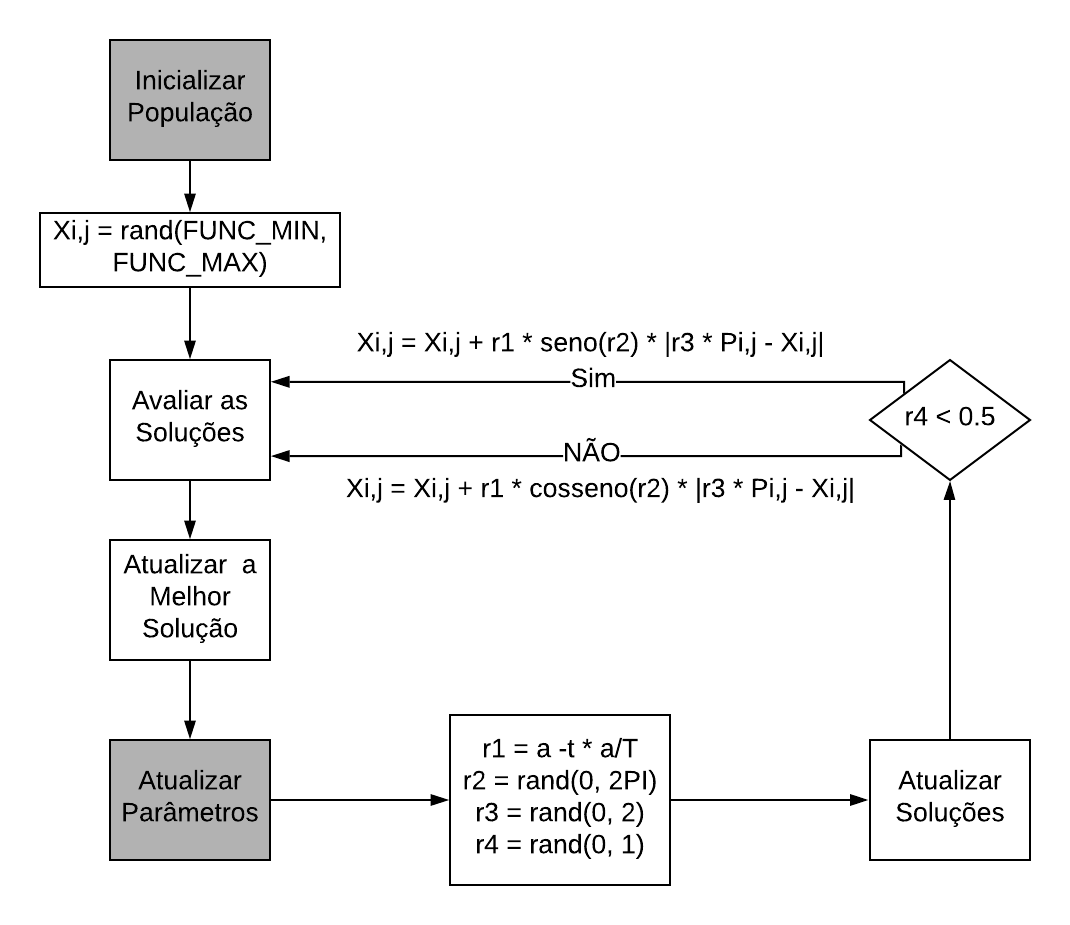
\includegraphics[width=0.7\linewidth]{figuras/Diagrama_SCA.png}
    \captionof{figure}{Diagrama de Blocos do SCA}
    \label{fig:SCA}
    \source{Própria autora.}
}



%Com muita intensificação e pouca diversificação o algoritmo pode convergir rapidamente para uma solução ótima, mas que pode não ser o ótimo global \cite{sahib}. No contrário, pouca intensificação e muita diversificação pode causar convergência lenta, mas prevenindo o algoritmo de ficar preso em ótimos locais \cite{sahib}. Sendo assim, implementar uma meta-heurística com um balanço apropriado entre intensificação e diversificação é essencial e pode levar a um desempenho ótimo \cite{sahib}.

% \section{Problemas do Mundo Real e Funções Benchmark}

% Em geral, problemas \ sem restrições podem ser classificados em duas categorias: funções de teste, ou funções \textit{benchmark}, e problemas do mundo real \cite{jamil}. As funções de teste são problemas artificiais e podem ser usadas para avaliar o comportamento de um algoritmo em situações diversas e difíceis \cite{jamil}. Os problemas artificiais podem incluir mínimos globais únicos, únicos ou múltiplos mínimos globais na presença de muitos mínimos locais, vales longos e estreitos, efeitos de espaço nulo e superfícies planas \cite{jamil}. Esses problemas podem ser facilmente manipulados e modificados para testar os algoritmos em diversos cenários \cite{jamil}. Alguns exemplos de funções \textit{benchmark} são as funções Schaffer, Rastrigin, Griewank e Rosenbrock. 

% Por outro lado, os problemas do mundo real se originam de campos diferentes como física, química, engenharia, matemática, entre outros \cite{jamil}. Esses problemas são difíceis de manipular e podem conter expressões algébricas ou diferenciais complicadas e podem exigir uma quantidade significativa de dados para compilar \cite{jamil}. 

\section{Problema de Predição da Estrutura de Proteínas}
\label{sec:psp}

Proteínas são estruturas básicas que compõem todos os seres vivos, e são compostas por uma cadeia de aminoácidos que são ligados entre si através de ligações peptídicas \cite{parpinelli}. Nas ligações peptídicas, o grupo carboxila de um aminoácido se une ao grupo amino de outro aminoácido e a molécula de água produzida \cite{jana4}. A cadeia resultante, que forma a proteína, é referida como uma cadeia peptídica e é utilizada para formar uma longa sequência de aminoácidos \cite{jana4}. As proteínas são dobradas em uma estrutura única durante o processo de síntese e, suas funções biológicas são determinadas a partir dessas estruturas, tendo um papel importante no desenvolvimento de medicamentos, predição de doenças e outras aplicações \cite{jana2}.

A maioria das estruturas proteicas são determinadas utilizando métodos de cristalografia de raios-X e ressonância magnética nuclear (NMR), entretanto, esses métodos nem sempre são viáveis para se conduzir - por isso, pesquisadores foram motivados a desenvolver métodos computacionais para determinar a estrutura de proteínas, a partir de dois passos: em primeiro lugar, um modelo físico correspondente a uma função de energia da proteína é desenvolvido e, em segundo lugar, o mínimo global da função de energia é obtido usando um algoritmo de otimização \cite{jana2}. Um desses modelos físicos é o modelo AB \textit{off-lattice}, que será utilizado neste trabalho. É importante destacar que o problema PSP baseado no modelo \textit{off-lattice} 2D e 3D é um problema de otimização complexo, NP-\textit{hard} \cite{jana4}.

\subsection{Modelo \textit{off-lattice} 2D-AB}

Nesse modelo as sequências de proteínas são compostas por apenas dois tipos de monômeros (moléculas que se combinam com outras para formar um polímero \cite{rudin}), classificados a partir das suas afinidades com a água: "A" \- para aminoácidos hidrofóbicos e "B" \- para aminoácidos hidrofílicos (ou polares) - além disso, os monômeros possuem uma unidade de comprimento de distância entre eles, de modo que cada monômero é conectado com o próximo na cadeia através de uma ligação que forma um ângulo relativo ao seu antecessor \cite{parpinelli}.

No modelo AB, uma proteína composta de \textit{n} monômeros necessita de \textit{n - 2} ângulos para ser representada, e esses ângulos são definidos no intervalo $[-\pi, \pi]$ \cite{parpinelli}. Um exemplo de representação pode ser vista na figura \ref{fig:exemploProteina}, onde tem-se uma sequência com oito aminoácidos e seis ângulos.

{
    \centering
    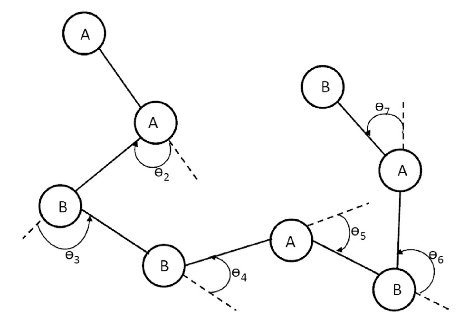
\includegraphics[width=0.6\linewidth]{figuras/exemploProteina.png}
    \captionof{figure}{Representação do modelo \textit{off-lattice} 2D-AB para a sequência proteica AABBABAB}
    \label{fig:exemploProteina}
    \source{\cite{jana2}}
}

O modelo também define valores de energia para os monômeros: "A" \- possui energia 1 e "B" \- possui energia -1 e, considerando dois monômeros genéricos \textit{i} e \textit{j}, e os tipos $\xi_i$ e $\xi_j$, tem-se que a interação entre os monômeros leva a valores diferentes de energia potencial \textit{C}: valores positivos representam atração e valores negativos, repulsão - ligações "AA" \- têm energia 1 (atração forte); ligações "BB" \- têm energia $\frac{1}{2}$ (atração fraca); e ligações "AB" \- ou "BA" \- têm energia $-\frac{1}{2}$ (repulsão fraca) \cite{parpinelli}.

A energia \textit{E} da estrutura de uma proteína com \textit{n} monômeros é dada pela equação \ref{eq:proteinE} \cite{parpinelli}.

\begin{equation}
    E(\Vec{\theta}, \Vec{\xi}) = \sum_{i=1}^{n-1} V_1(\theta_i) + \sum_{i=1}^{n-2} \sum_{j=i+2}^{n} V_2(d_{ij}, \xi_i, \xi_j)
\label{eq:proteinE}
\end{equation}

Essa equação postula dois tipos de energias potenciais intermoleculares, $V_1$ e $V_2$, onde a primeira representa potenciais \textit{backbone}, depende apenas do ângulo entre monômeros e é calculada a partir da equação \ref{eq:proteinV1}; e a segunda, definida pela equação \ref{eq:proteinV2}, representa a energia potencial presente nas interações sem limites e é conhecida como o potencial \textit{Lennard-Jones} \cite{parpinelli}.

\begin{equation}
    V_1(\theta_i) = \frac{1}{4} * (1 - cos(\theta_i))
\label{eq:proteinV1}
\end{equation}

\begin{equation}
    V_2(d_{ij}, \xi_i, \xi_j) = 4 * (d_{ij}^{-12} - C(\xi_i, \xi_j) * d_{ij}^{-6})
\label{eq:proteinV2}
\end{equation}

onde 

\begin{equation}
    C(\xi_i, \xi_j) = \frac{1}{8 * (1 + \xi_i + \xi_j + 5 * \xi_i * \xi_j)}
\label{eq:proteinC}
\end{equation}

A equação \ref{eq:proteinC} é a energia potencial da interação entre os monômeros \textit{i} e \textit{j}, e $d_{ij}$ é a distância entre esses monômeros na cadeia, de modo que $i < j$ \cite{parpinelli}.

\chapter{Revisão da Literatura} \label{chap2}

Neste capítulo será apresentado o Mapeamento Sistemático da Literatura (MSL) realizado, com intuito de proporcionar uma visão geral da área de pesquisa deste trabalho, que envolve a aplicação de métodos de randomização (diferentes do Uniforme) em meta-heurísticas. A metodologia utilizada para o desenvolvimento deste mapeamento é baseada nas diretrizes propostas por \cite{petersen}. O trabalho foi realizado no mês de Abril do ano de 2019.

\section{Método de Busca}

Para a execução da busca, foi definida uma string de busca, apresentada na tabela \ref{tab:string}. Inicialmente, alguns termos de interesse foram estabelecidos, como: \textit{probability distribution}, \textit{randomization methods} e a versão em inglês britânico do mesmo termo; assim também como \textit{chaotic series}, \textit{chaotic sequence} e \textit{chaotic map}. Essas expressões foram utilizadas para encobrir as possíveis representações utilizadas para os diferentes métodos de randomização, incluindo mapas caóticos. Além disso, o termo \textit{metaheuristic} foi utilizado para representar o tipo de algoritmo que estamos buscando, que neste caso, são as meta-heurísticas.

\begin{table}[!htpb]
    \centering
    \begin{tabular}{|c|}
    \hline
        ("randomization methods" \- OR "randomisation methods" \- OR "probability distribution" \- \\OR "chaotic series" \- OR "chaotic sequence" \- OR "chaotic map") AND metaheuristic \\
    \hline
    \end{tabular}
    \caption{String de Busca}
    \label{tab:string}
\end{table}


A \textit{string} definida foi executada em três mecanismos de busca distintos: Engineering Village, Scopus e IEEE Xplore. Como pode-se observar na tabela \ref{tab:resultado}, ao fazer a busca, reunindo o resultado de todas as bases, foi encontrado um total de 222 artigos, de onde destes apenas 143 estavam disponíveis na íntegra.

\begin{table}[!htpb]
    \centering
    \begin{tabular}{c|c} % <-- Alignments: 1st column left, 2nd middle and 3rd right, with vertical lines in between
      \textbf{Mecanismo} & \textbf{Quantidade} \\
      \hline
      Engineering Village & 26\\
      Scopus & 71\\
      IEEE Xplore & 125\\
      \hline
      Total & 222\\
      Disponíveis & 143\\
      Considerados & 43\\
    \end{tabular}
    \caption{Resultados dos Mecanismos de Busca}
    \label{tab:resultado}
\end{table}

\section{Seleção dos Estudos Primários}

Após a realização da busca, foi feito o \textit{download} dos 143 artigos disponíveis e os mesmos passaram por um processo de seleção com o intuito de fazer a identificação dos estudos primários. Neste processo, foram analisados o título, as palavras-chave, o \textit{abstract} e quando necessário, caso existisse dúvidas em relação a inclusão ou exclusão, a introdução e a conclusão dos artigos. Foram aplicados os seguintes critérios de inclusão:

\begin{itemize}
    \item Artigos completos, de 4 páginas ou mais;
    %\item Artigos que apresentam a inclusão de um método de randomização como melhoria em alguma meta-heurística.
    \item Artigos que apresentam uma nova versão de alguma meta-heurística, utilizando um método de randomização diferente do original.
\end{itemize}


Os critérios de exclusão aplicados foram:

\begin{itemize}
    \item Artigos publicados fora do período de 2009 até 2019;
    \item Artigos duplicados;
    \item Artigos que não propõem uma nova versão de uma meta-heurística, apenas a utilizam para aplicação em algum problema;
    \item Artigos que apresentam algoritmos que não são baseados em população;
    \item Artigos que apresentam como método de randomização apenas a distribuição Uniforme.
\end{itemize}

Após a aplicação dos critérios de inclusão e exclusão mencionados, restaram 43 artigos, como visto na tabela \ref{tab:resultado}. As referências dos artigos podem ser encontradas na seção de Bibliografia deste trabalho, indicados pelo símbolo \textit{*}. Após esse processo, foi realizado um processo de extração e análise dos dados coletados, apresentado na seção \ref{sec:analise}.

\section{Questões de Pesquisa}

Para compreender melhor os trabalhos encontrados no mapeamento, foram definidas algumas questões de pesquisa a serem respondidas:

\begin{itemize}
    \item \textbf{QP1} - Qual o método de randomização que o estudo utiliza? 
    \item \textbf{QP2} - Qual foi o motivo para realizar a adaptação do algoritmo com este método de randomização?
    \item \textbf{QP3} - Em que parte do algoritmo este método de randomização foi aplicado?
\end{itemize}

\section{Análise dos Resultados}
\label{sec:analise}

Nessa seção serão apresentados os resultados do Mapeamento Sistemático da Literatura, começando com uma visão geral, com informações pertinentes sobre os estudos; e depois apresentando as respostas para as questões de pesquisa propostas. É válido destacar que dos 43 estudos inclusos, 5 não serão incluídos nas análises e nos gráficos - isto porque esses estudos são repetidos, possuindo a mesma abordagem de estudos já inclusos, mudando apenas os problemas aos quais essas abordagens são aplicadas.


%%%%%%%%%%%%%%%%%%%%%%%%%%%%%%%%%%%%%%%%%%%%%%%%%%%
\nocite{*}
%%%%%%%%%%%%%%%%%%%%%%%%%%%%%%%%%%%%%%%%%%%%%%%%%%%


\subsection{Visão Geral}

A primeira característica analisada nos artigos foi o ano de publicação dos mesmos. Como pode-se observar na figura \ref{fig:grafAnos}, tem-se que a quantidade de artigos abordando o tema de diferentes métodos de randomização em meta-heurísticas têm crescido ao longo dos anos, desde 2011 até 2018. Sendo assim, pode-se concluir que o interesse por essa área têm aumentado, e possui a tendência de aumentar ainda mais. Esse fato também nos mostra que cada vez mais pesquisadores têm percebido a importância da randomização para as meta-heurísticas e decidido verificar quais são os melhores métodos para serem utilizados. Além disso, o ano de 2019 teve apenas 3 artigos publicados até então, mas precisamos levar em consideração que apenas os três primeiros meses do ano foram contabilizados no mapeamento - dessa forma, mais artigos podem ser publicados ao longo do ano.

{
    \centering
    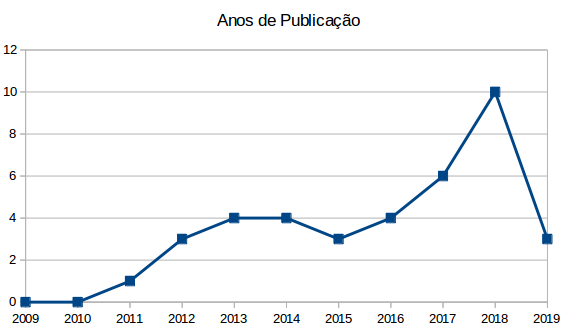
\includegraphics[width=0.7\linewidth]{figuras/graficoAnos.png}
    \captionof{figure}{Anos de Publicação dos Estudos}
    \label{fig:grafAnos}
    \source{Própria autora.}
}

Outro ponto interessante de se analisar é qual o algoritmo que os estudos utilizaram. Um artigo, do \cite{mitic2}, apresentou diversos algoritmos, como o \textit{Bat Algorithm, Firefly Algorithm, Accelerated Particle Swarm Optimization} e \textit{Grey Wolf Optimizer}. Todos os outros estudos realizaram a adaptação de apenas uma única meta-heurística. Como pode-se observar na figura \ref{fig:grafAlgoritmos}, diversos algoritmos foram utilizados. Entretanto, o\textbf{ \textit{Firefly Algorithm}} se destacou pela sua popularidade, sendo abordado em 8 estudos, seguido do \textbf{\textit{Bat Algorithm}} e do \textbf{\textit{Grey Wolf Optimizer}}, com 4 estudos; o \textit{Cuckoo Search Algorithm} foi usado em três artigos; e em sequência, o \textit{Imperialist Competitive Algorithm} e o \textit{Colliding Bodies Algorithm}, que foram utilizados em 2 estudos. A categoria Outros do gráfico engloba todos os outros algoritmos, que apareceram apenas uma vez nos artigos. Essa categoria inclui os seguintes algoritmos: \textit{Real-Coded Chemical Reaction Optimization}, \textit{Backtracking Search Optimization Algorithm}, \textit{Grasshopper Optimization Algorithm}, \textit{Dragonfly Algorithm}, \textit{Fruit Fly Optimization Algorithm}, \textit{League Championship Algorithm}, \textit{Accelerated Particle Swarm Optimization}, \textit{Intelligent Tuned Harmony Search}, \textit{Crow Search Algorithm}, \textit{Salp Swarm Algorithm}, \textit{Darwinian Particle Swarm Optimization}, \textit{Symbiotic Organisms Search}, \textit{Wind Driven Optimization}, \textit{Particle Swarm Optimization}, \textit{Self-Adaptive Differential Evolution}, \textit{Monarch Butterfly Optimization Algorithm}, \textit{Artificial Bee Colony} e \textit{Whale Optimization Algorithm}.

{
    \centering
    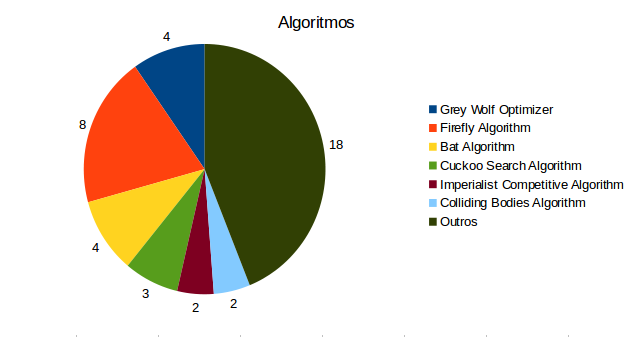
\includegraphics[width=0.9\linewidth]{figuras/graficoAlgoritmos2.png}
    \captionof{figure}{Algoritmos Utilizados nos Estudos}
    \label{fig:grafAlgoritmos}
    \source{Própria autora.}
}


%     \fontsize{6}{11}\selectfont{
%     \centering
%     \begin{longtable}{p{5cm}|p{3cm}} % <-- Alignments: 1st column left, 2nd middle and 3rd right, with vertical lines in between
%     \tiny
%   \textbf{Algoritmo} & \textbf{Quantidade} \\
%       \hline
%       Real-Coded Chemical Reaction Optimization & 1\\
%       \hline
%       Grey Wolf Optimizer & 4\\
%       \hline
%       Backtracking Search Optimization Algorithm & 1\\
%       \hline
%       Firefly Algorithm & 8\\
%       \hline
%       Bat Algorithm & 4\\
%       \hline
%       Cuckoo Search Algorithm & 3\\
%       \hline
%       Imperialist Competitive Algorithm & 2\\
%       \hline
%       Grasshopper Optimization Algorithm & 1\\
%       \hline
%       Dragonfly Algorithm & 1\\
%       \hline
%       Colliding Bodies Algorithm & 2\\
%       \hline
%       Fruit Fly Optimization Algorithm & 1\\
%       \hline
%       League Championship Algorithm & 1\\
%       \hline
%       Accelerated Particle Swarm Optimization & 1\\
%       \hline
%       Intelligent Tuned Harmony Search & 1\\
%       \hline
%       Crow Search Algorithm & 1\\
%       \hline
%       Salp Swarm Algorithm & 1\\
%       \hline
%       Darwinian Particle Swarm Optimization & 1\\
%       \hline
%       Symbiotic Organisms Search & 1\\
%       \hline
%       Wind Driven Optimization & 1\\
%       \hline
%       Particle Swarm Optimization & 1\\
%       \hline
%       Self-Adaptive Differential Evolution & 1\\
%       \hline
%       Monarch Butterfly Optimization Algorithm & 1\\
%       \hline
%       Artificial Bee Colony & 1\\
%       \hline
%       Whale Optimization Algorithm  & 1\\
%       \hline
%       \caption{Resultados do jDE}
%     \label{tab:features}
%     \end{longtable}
%     }

\subsection{Métodos de Randomização (QP1)}

Para responder a primeira questão de pesquisa, foram levantadas as distribuições utilizadas pelos autores ao adaptarem as meta-heurísticas apresentadas nos artigos. No total, 33 métodos de randomização foram encontrados. Na figura \ref{fig:grafDistribuicoes} tem-se os tipos de distribuições que foram usadas e as suas respectivas ocorrências, sendo que a soma total do gráfico se apresenta superior ao número de artigos, visto que na maioria dos artigos os autores utilizaram mais de um método nas abordagens. Como pode-se perceber, os mapas caóticos foram de longe o tipo de distribuição mais utilizada. Isso mostra como há um grande interesse na área pela aplicação de Teoria do Caos em algoritmos de otimização, e também que os mesmos foram selecionados por terem obtido um impacto positivo na literatura, mostrando como podem ser utilizados para se obter um melhor desempenho. Além dos mapas, tem-se a distribuição Gaussiana, com 5 ocorrências; o Levy Flights, com 4; e as distribuições de Cauchy, Exponencial, de Rayleigh, Beta, Fat-tailed e de Levy, com 1 ocorrência cada.

{
    \centering
    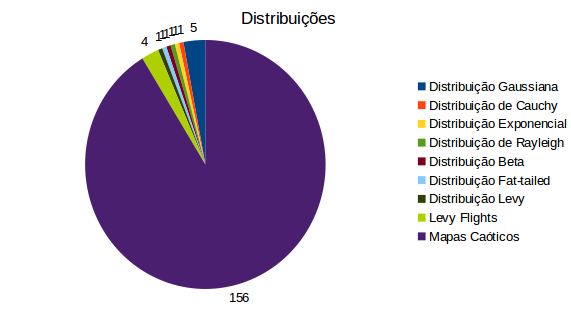
\includegraphics[width=0.7\linewidth]{figuras/graficoDistribuicoes.png}
    \captionof{figure}{Distribuições Utilizadas nos Estudos}
    \label{fig:grafDistribuicoes}
    \source{Própria autora.}
}

Na tabela \ref{tab:grafMapas} tem-se de forma mais específica cada mapa que foi usado nos estudos, onde a soma total representa as 156 ocorrências totais dos mapas caóticos. O mais utilizado foi o \textbf{mapa Logístico}, com 22 ocorrências. Isso não é surpreendente se for levado em consideração que ele é o mapa caótico mais conhecido, além de ser um mapa de simples implementação. Em sequência, tem-se o \textbf{mapa Sinusoidal}, com 17 ocorrências; o \textbf{mapa Gauss}, com 16; e assim por diante. 

%o mapa Tent, com 15; o mapa Circle, com 14; o mapa Piecewise, com 11; e o mapa Singer, com 10. Além disso tem-se outros mapas com menos ocorrências, como o Chebyshev, Iterativo, Sine, Liebovitch, de Intermitência, Hénon, Tinkerbell, Sinus, Burgers e por fim, outros que apareceram em apenas um artigo, como o mapa Beta, Sawtooth, ICMIC, Arnold Cat, Delayed Logistic, Dissipative Standard, Ikeda, Lozi e Sinai. 

{\tiny
\begin{table}[!htpb]
    \centering
    \begin{tabular}{c|c} % <-- Alignments: 1st column left, 2nd middle and 3rd right, with vertical lines in between
      \textbf{Mapa} & \textbf{Ocorrências} \\
      \hline
      Mapa Beta & 1\\
      \hline
    Mapa Logístico & 22\\
    \hline
    Mapa Chebyshev & 9 \\
    \hline
    Mapa Burgers & 2\\
    \hline
    Mapa Circle	 & 14\\
    \hline
    Mapa Sinusoidal	 & 17\\
    \hline
    Mapa Gauss & 16\\
    \hline
    Mapa Iterativo & 8\\
    \hline
    Mapa Piecewise & 11\\
    \hline
    Mapa Sine & 8\\
    \hline
    Mapa Singer	 & 10\\
    \hline
    Mapa Tent & 15\\
    \hline
    Mapa de Intermitência & 4\\
    \hline
    Mapa Liebovitch	& 5\\
    \hline
    Mapa Sawtooth & 1\\
    \hline
    Mapa Hénon & 2\\
    \hline
    Mapa Tinkerbell	 & 2\\
    \hline
    Mapa ICMIC & 1\\
    \hline
    Mapa Sinus & 2\\
    \hline
    Mapa Arnold Cat	& 1\\
    \hline
    Mapa Delayed Logistic & 1\\
    \hline
    Mapa Dissipative Standard & 1\\
    \hline
    Mapa Ikeda & 1\\
    \hline
    Mapa Lozi & 1\\
    \hline
    Mapa Sinai & 1\\
    \end{tabular}
    \caption{Mapas Utilizados nos Estudos}
    \label{tab:grafMapas}
\end{table}
}

% {
%     \centering
%     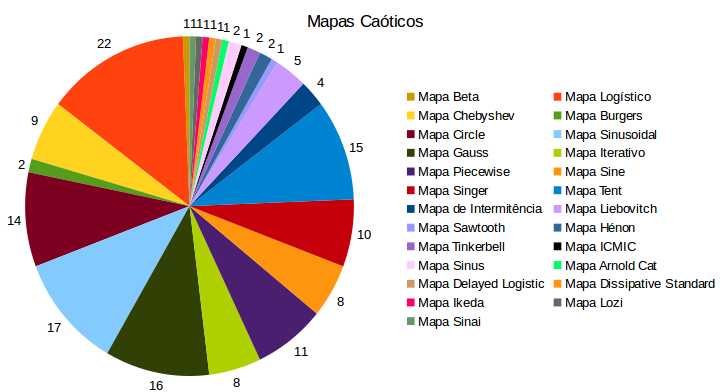
\includegraphics[width=1.0\linewidth]{figuras/graficoMapas.png}
%     \captionof{figure}{Mapas Utilizados nos Estudos}
%     \label{fig:grafMapas}
%     \source{Própria autora.}
% }

Além disso, as distribuições encontradas foram classificadas de acordo com a sua finalidade quando aplicadas à algoritmos de otimização: algumas intensificam o espaço de busca, outras diversificam e outras ainda podem apresentar ambas as finalidades - de acordo com os parâmetros utilizados na distribuição. Por exemplo, a distribuição Gaussiana possui dois parâmetros: a média e o desvio-padrão. Quando o desvio-padrão assume um valor pequeno, a distribuição realiza uma intensificação, e quando assume um valor grande, realiza uma diversificação, como pode-se visualizar na figura \ref{fig:Gaussiana}. 

Essa mesma situação ocorre também com algumas outras distribuições como a Cauchy, onde quanto maior o parâmetro de escala mais a distribuição diversifica; a Exponencial, onde acontece a mesma coisa com seu parâmetro de \textit{rate}; a de Rayleigh, onde ocorre a mesma situação com o parâmetro de escala; a distribuição Beta, que quando possui seus parâmetros de forma igual a 1, diversifica o espaço de busca, e caso contrário, intensifica; e por fim o Levy Flights, que por utilizar a distribuição de Levy, diversifica quando o parâmetro de escala é grande e intensifica quando o parâmetro de escala é pequeno. As outras distribuições, os chamados mapas caóticos, também possuem parâmetros. Entretanto, esses parâmetros são responsáveis apenas pelo comportamento caótico exibido pelos mesmos, sendo assim, os valores aplicados a eles são fixos e retirados da literatura.

{
    \centering
    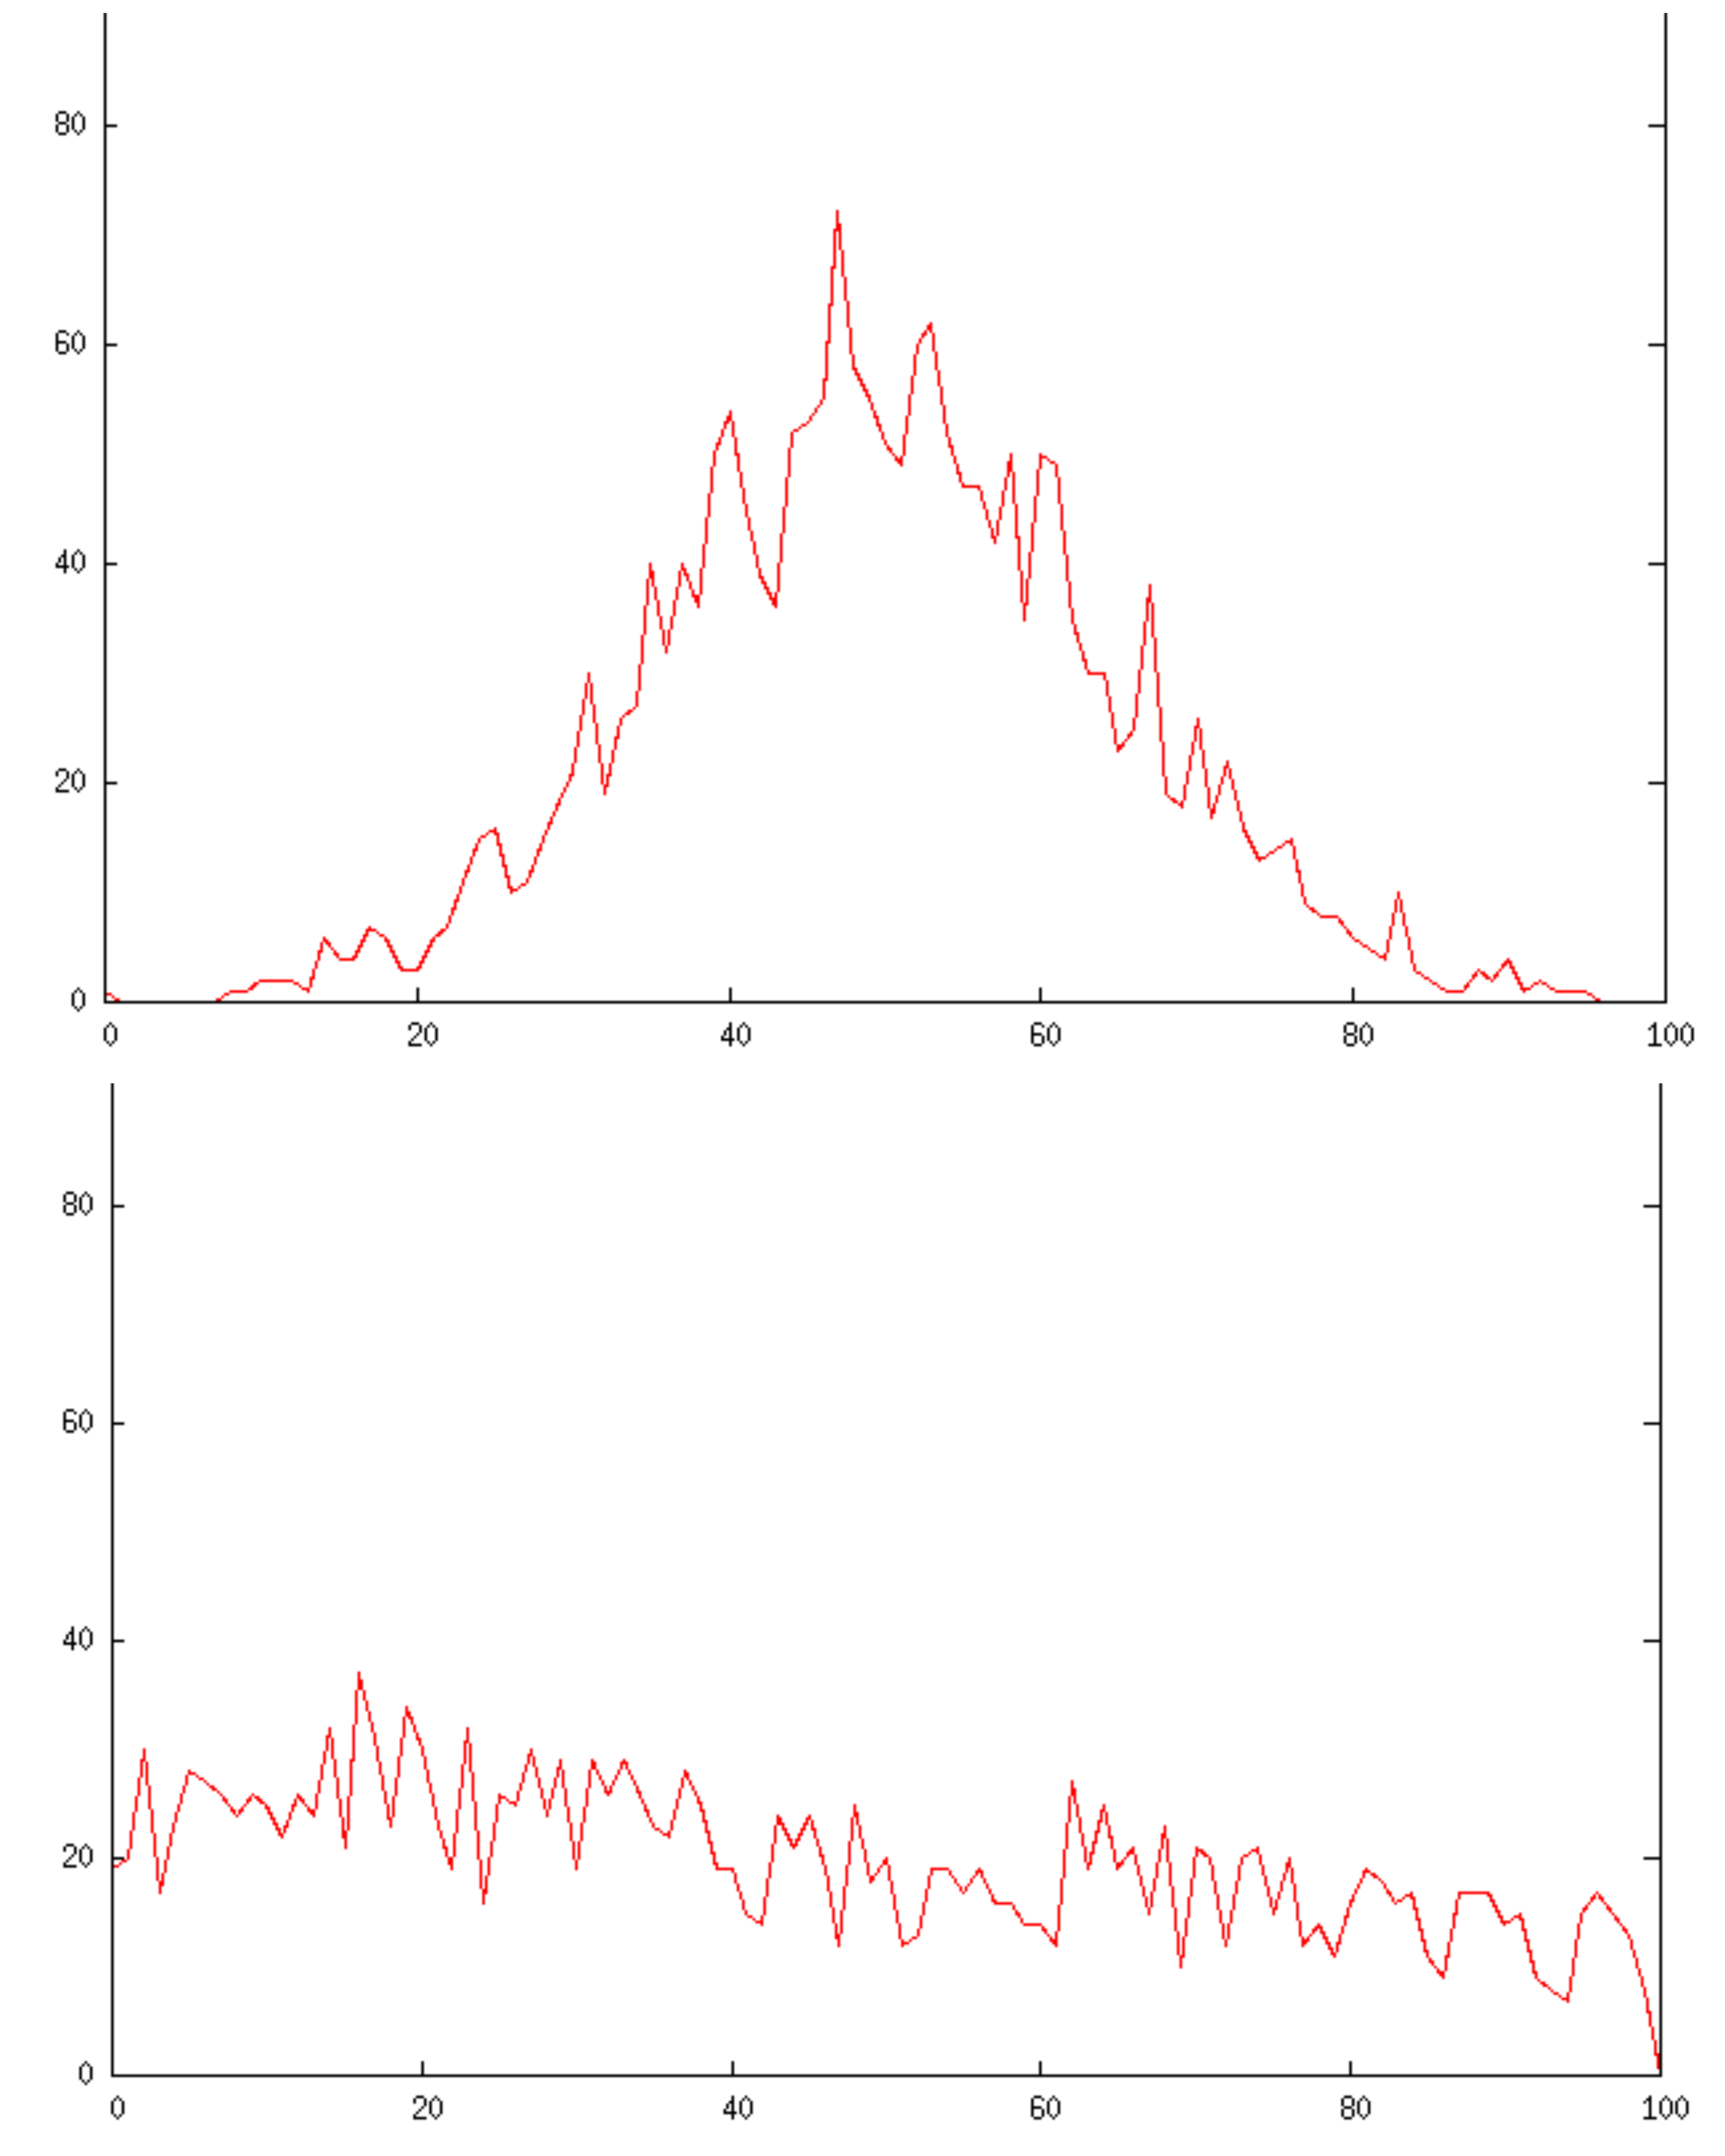
\includegraphics[width=0.7\linewidth]{figuras/gaussian.png}
    \captionof{figure}{Representação 1D da Distribuição Gaussiana com Diferentes Desvios-padrões}
    \label{fig:Gaussiana}
    \source{Própria autora.}
}

Ademais, alguns mapas caóticos apresentaram a característica de intensificação, como o Mapa Beta, Logístico, Circle, Sinusoidal, Gauss, Chebyshev, Sine e Singer; e outros, apresentaram a característica de diversificação, como o Mapa Iterativo, Piecewise e Tent. 

\subsection{Motivação (QP2)}

Diversas questões foram apontadas como motivação para realizar a adaptação dos algoritmos com os seus respectivos métodos de randomização, sendo que a maioria dos estudos apresentou mais de uma motivação. Algumas motivações mais óbvias foram citadas, como por exemplo que a adaptação foi realizada para melhorar o desempenho do algoritmo de forma geral, melhorando sua eficiência e capacidade de convergência - citada por um total de 15 artigos. Outro ponto apresentado foi o impacto positivo que mapas caóticos tiveram na literatura, citado por 3 estudos. Ademais, foram citados por artigos individuais a necessidade de se estudar o impacto no resultado final do algoritmo, de diferentes distribuições como funções de pertubação, no trabalho de \cite{yu}; e foi citado como motivo no estudo de \cite{ismail}, que a distribuição Levy foi utilizada por ser a forma mais rápida de se encontrar um alvo randomicamente escondido.

As motivações restantes podem ser classificadas em quatro categorias - a análise de diversificação, a intensificação, a diversificação e o balanço entre busca global/local, como pode-se observar na figura \ref{fig:grafMotivacoes}. A categoria de análise de diversidade se refere ao trabalho de \cite{senserik2}, que apontou a necessidade de se pesquisar o impacto que séries caóticas possuem na diversidade da população. A categoria de intensificação engloba artigos que apontaram a inclusão de métodos de randomização como forma de intensificar o processo de busca, acelerando a velocidade de convergência do algoritmo. Já a categoria de diversificação engloba estudos que fizeram essa inclusão para diversificar a população, com objetivo de evitar problemas como a convergência prematura e estagnação em ótimos locais. Por fim, a categoria de balanço entre busca global/local inclui artigos que tiveram como motivação melhorar o balanço do algoritmo entre busca local (intensificação) e busca global (diversificação).

{
    \centering
    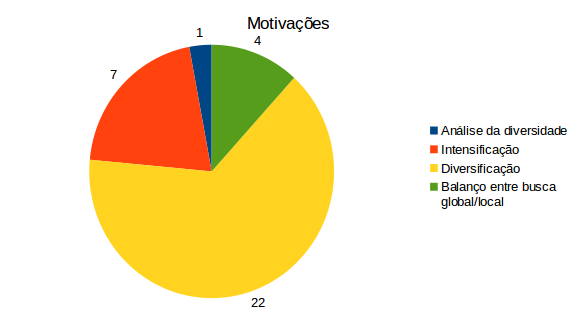
\includegraphics[width=0.7\linewidth]{figuras/graficoMotivacoes.png}
    \captionof{figure}{Categorias de Motivações Apresentadas nos Estudos}
    \label{fig:grafMotivacoes}
    \source{Própria autora.}
}

Pode-se perceber através das motivações que realizar a mudança de uma distribuição Uniforme para outra distribuição pode impactar imensamente os resultados do algoritmo - melhorando seu desempenho, seu balanço entre intensificação e diversificação, e evitando problemas como a convergência lenta e prematura, e a estagnação em ótimos locais. Não só isso, mas também pode-se observar na figura \ref{fig:grafMotivacoes} que a diversificação é uma das maiores motivações para a aplicação de diferentes métodos de randomização nos algoritmos - isso se dá pelo fato de que quer-se sempre manter a diversidade presente até as últimas iterações, visto que todos esses algoritmos populacionais sofrem de problemas como a convergência prematura.

% Esse motivo foi abordado nos estudos de \cite{farshin}, \cite{coelho2}, \cite{saida}, \cite{mortazavi}, \cite{wang}, \cite{sayed}, \cite{mitic2}, \cite{turgut}, \cite{ahmed}, \cite{talahari}, \cite{saeed}, \cite{ayala}, \cite{saeed2}, \cite{ding} e \cite{chou3}.

\subsection{Aplicação (QP3)}

As respostas da terceira e última questão de pesquisa mostram que, na maioria dos casos, os métodos de randomização são aplicados em pontos específicos dos algoritmos. Por exemplo, no trabalho de \cite{yu} as distribuições são incorporadas no operador de busca de vizinhança e na operação de decomposição; em \cite{alireza} o mapa caótico é incorporado no fator de escala relacionado ao processo de mutação; no estudo de \cite{coelho}, é incorporado no coeficiente de absorção e no parâmetro de randomização; no artigo de \cite{farshin}, é incorporado na função de atualização dos vetores de coeficiente; em \cite{liang} é incorporado nos parâmetros de sonoridade e taxa de emissão de pulso; em \cite{lin} é incorporado no Levy Flights proposto para substituir o Random Walk; em \cite{coelho2} a distribuição é inserida no parâmetro de randomização $\alpha$; em \cite{wang} é inserida no tamanho do passo $\alpha$; em \cite{kaveh} as distribuições são inseridas de três formas distintas: primeiramente, na probabilidade de mudança do algoritmo; em segundo, são usadas para selecionar as variáveis candidatas para regeneração; e em terceiro, são usadas na regeneração da variável selecionada. 

No trabalho de \cite{mitic} são inseridas em um novo parâmetro chamado $\alpha$, usado para a geração de origens de comida; em \cite{bingol} são incorporadas de seis formas diferentes, todas envolvendo os parâmetro r, r1 e r2 do algoritmo; em \cite{mitic2} são incorporadas no valor randômico r e no parâmetro de exploração C; em \cite{coelho4} a distribuição é incorporada nos parâmetros de consciência e tamanho do voo; no artigo de \cite{ahmed} são inseridas no parâmetro c3; em \cite{gandomi2} são inseridas nos coeficientes de absorção de luz e atratividade; em \cite{coelho3} o mapa caótico é inserido no coeficiente de absorção de luz; no trabalho de \cite{wood} o mapa caótico é incorporado no fator de escala e a distribuição \textit{fat-tailed} no fator de ajustamento estocástico; em \cite{talahari} são incorporados nos parâmetros randômicos da equação de assimilação; em \cite{ayala}, são incorporados nos parâmetros de controle na fase de mutualismo; em \cite{ismail}, a distribuição foi incorporada na função de atualização de posição das partículas; em \cite{saeed2} foram inseridas na função de mutação e de atualização de posição; em \cite{ding} o mapa Logístico foi aplicado nas estratégias de \textit{encircling prey} e \textit{bubble-net attacking} e o mapa Sinusoidal na mutação; em \cite{mortazavi} onde foram aplicados em uma porcentagem de colônias revoltadas; e em \cite{saeed} onde foram aplicados na funções de atualização, mutação e geração de novos indivíduos para a próxima geração.

A segunda maioria dos casos aplica as distribuições em todos os parâmetros do algoritmo que necessitam de randomização. Como o trabalho de \cite{gandomi}; de \cite{sayed}; de \cite{turgut}; de \cite{ayala2}, onde as distribuições são incorporadas em todos os parâmetros de controle: R, T, c, g e $\alpha$; de \cite{senserik2}; de \cite{jaddi};e o de \cite{feng}, onde se utiliza a distribuição gaussiana na atualização do pior indivíduo e as séries caóticas em todos os outros pontos de randomização.

E além desses casos, os métodos também foram aplicados no mecanismo de balanço entre diversificação e intensificação do algoritmo, como no caso do trabalho de \cite{saxena}, onde o mapa Beta é aplicado no vetor de controle responsável por realizar a busca global e local ao longo das iterações do GWO; no trabalho de \cite{saxena2}, onde os mapas são aplicados no parâmetro c, de redução da zona de conforto, o qual é o mecanismo de ponte que liga a intensificação e a diversificação do algoritmo; e no trabalho de \cite{oliveira} onde foram aplicados no vetor de controle e no parâmetro C.

Alguns artigos mostraram que os métodos também foram incorporados na geração da população inicial das meta-heurísticas, como no trabalho de \cite{saida}; no artigo de \cite{suresh}, onde o mapa caótico é aplicado tanto na geração da população inicial como na velocidade de \textit{drift} dos agentes; no estudo de \cite{abro}; e no trabalho de \cite{chou3} onde o mapa Logístico é utilizado na inicialização da população, o mapa Gauss no parâmetro de atratividade e o Levy Flights para realizar a movimentação das \textit{fireflies}.

Um ponto importante, que recebe destaque, é a forma como o trabalho de \cite{wood} realizou a aplicação da distribuição no algoritmo. No estudo, o \textit{Cuckoo Search Algorithm} é adaptado com várias melhorias, uma delas sendo na parte de troca do algoritmo, mais especificamente na equação que gera novos indivíduos para substituir indivíduos com \textit{ranking} baixo ou médio \cite{wood}. Nessa equação, existe um parâmetro \textit{F}, chamado de fator de ajuste estocástico, que é retirado de uma distribuição \textit{fat-tailed}, amostrada através de uma janela de amostragem entre os limites de probabilidade inferiores e superiores, que variam dinamicamente conforme as iterações progridem \cite{wood}.
Sendo assim, o campo distante de randomização é mais amostrado nas iterações iniciais (fazendo o algoritmo realizar uma diversificação / busca global no espaço de solução) e o campo próximo é mais amostrado nas iterações finais (fazendo o algoritmo realizar uma intensificação / busca local no espaço de solução) \cite{wood}. Ou seja, o autor utiliza a distribuição como uma forma de favorecer os processos de intensificação e diversificação do espaço de busca.

Finalmente, pode-se concluir a partir da análise desses estudos, que o local de aplicação dos métodos de randomização pode depender do algoritmo, sendo aplicado em pontos específicos do mesmo. Entretanto, os métodos também podem ser aplicados em locais que favoreçam a intensificação ou a diversificação do algoritmo, como na geração da população inicial; além de locais que envolvem o balanço entre a busca global e local, como os mecanismos de ponte.

% {
%     \centering
%     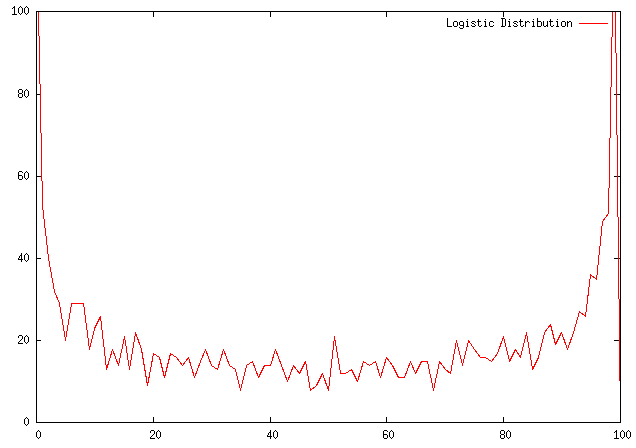
\includegraphics[width=0.7\linewidth]{figuras/logisticDistribution.png}
%     \captionof{figure}{Representação 1D da Distribuição Logística}
%     \label{fig:Gaussiana}
% }

% {
%     \centering
%     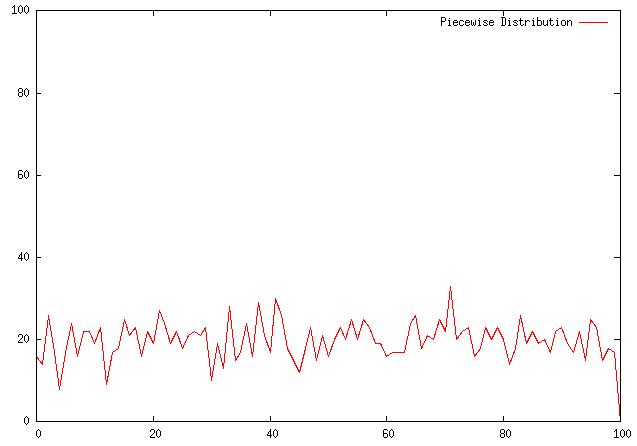
\includegraphics[width=0.7\linewidth]{figuras/piecewiseDistribution.png}
%     \captionof{figure}{Representação 1D da Distribuição Piecewise}
%     \label{fig:Gaussiana}
% }

    % \centering
    % \begin{longtable}{p{4cm}|p{4cm}|p{3cm}|p{3cm}} % <-- Alignments: 1st column left, 2nd middle and 3rd right, with vertical lines in between
    %   \textbf{Distribuição} & \textbf{Referências} & \textbf{Intensificação} & \textbf{Diversificação}\\
    %   \hline
    %   Distribuição Gaussiana & \cite{yu} & \checkmark  & \checkmark\\
    %   \hline
    %   Distribuição de Cauchy & \cite{yu} & \checkmark & \checkmark\\
    %   \hline
    %   Distribuição Exponencial & \cite{yu} & \checkmark & \checkmark\\
    %   \hline
    %   Distribuição de Rayleigh modificada & \cite{yu} & \checkmark  & \checkmark\\
    %   \hline
    %   Distribuição Beta & \cite{coelho2} & \checkmark & \checkmark\\
    %   \hline
    %   Levy Flights & \cite{lin} & \checkmark & \checkmark\\
    %   \hline
    %   Mapa Beta & \cite{saxena} & \checkmark &\\
    %   \hline
    %   Mapa Burgers & \cite{alireza} &- &-\\
    %   \hline
    %   Mapa Logístico & \cite{coelho}, \cite{lin}, \cite{saida}, \cite{mortazavi}, \cite{wang}, \cite{saxena2},\cite{gandomi}, \cite{wang2}, \cite{sayed} & \checkmark  & \\
    %   \hline
    %   Mapa Circle & \cite{farshin}, \cite{mortazavi}, \cite{wang}, \cite{saxena2}, \cite{gandomi}, \cite{wang2}, \cite{sayed} & \checkmark &\\
    %   \hline
    %   Mapa Sinusoidal & \cite{liang}, \cite{wang}, \cite{saxena2}, \cite{gandomi}, \cite{wang2}, \cite{sayed} & \checkmark&\\
    %   \hline
    %   Mapa de Gauss & \cite{mortazavi}, \cite{wang}, \cite{saxena2}, \cite{gandomi}, \cite{wang2}, \cite{sayed} &\checkmark &\\
    %   \hline
    %   Mapa Chebyshev & \cite{wang}, \cite{saxena2}, \cite{gandomi}, \cite{wang2}, \cite{sayed} & \checkmark &\\
    %   \hline
    %   Mapa Interativo & \cite{wang}, \cite{saxena2}, \cite{gandomi}, \cite{wang2}, \cite{sayed} &  & \checkmark\\
    %   \hline
    %   Mapa de Intermitência & \cite{wang}, \cite{gandomi}, \cite{wang2} &- &- \\
    %   \hline
    %   Mapa Liebovitch & \cite{wang}, \cite{gandomi}, \cite{wang2} &- &-\\
    %   \hline
    %   Mapa Piecewise  & \cite{wang}, \cite{saxena2}, \cite{gandomi}, \cite{wang2}, \cite{sayed} & & \checkmark\\
    %   \hline
    %   Mapa Seno & \cite{wang}, \cite{saxena2}, \cite{gandomi},\cite{wang2}, \cite{sayed} &\checkmark  &\\
    %   \hline
    %   Mapa Singer & \cite{wang}, \cite{saxena2}, \cite{oliveira}, \cite{gandomi}, \cite{wang2}, \cite{sayed} &\checkmark &\\
    %   \hline
    %   Mapa Tent & \cite{wang}, \cite{saxena2}, \cite{oliveira}, \cite{gandomi}, \cite{wang2}, \cite{sayed} && \checkmark\\
    %   \hline
    %   Mapa Sawtooth & \cite{gandomi} & - & -\\
    %   \hline
    %   \caption{Características das Distribuições Encontradas}
    % \label{tab:features}
    % \end{longtable}
    
% \chapter{Proposta}

% Neste capítulo será apresentado brevemente o problema e a solução proposta para o mesmo neste trabalho, além de um cronograma mostrando o planejamento das atividades para o TCC-2.

% \section{Problema}

% O problema abordado neste trabalho se refere ao fato de que a randomização possui extrema importância para as meta-heurísticas, e que além disso, tem-se a disposição diversos métodos de randomização que podem ser utilizados nos algoritmos, como a distribuição Uniforme, Gaussiana, e de Cauchy, assim também como os mapas caóticos, como o Logístico e de Kent. Entretanto, grande parte dos estudos não fazem uma análise de qual a melhor distribuição a se usar - acabam utilizando a distribuição Uniforme, por ser o gerador aleatório padrão de muitas linguagens.

% Não só isso, mas estudos como o de \cite{reese} mostram que o melhor gerador de números aleatórios para se utilizar depende não só do tipo de problema com o qual está se lidando, mas também do número de parâmetros, como o número de variáveis, a escolha da função, o espaço de busca e a acurácia desejada. Ou seja, utilizar o mesmo método de randomização para todos os tipos de problemas e em todas as partes do algoritmo que requerem randomização, como é feito na maioria dos casos, pode não ser a melhor opção.

% \section{Solução Proposta}
% \label{sec:solucao}
% Levando em consideração o problema apresentado, tem-se que a solução proposta para o mesmo envolve realizar uma análise do impacto que diferentes distribuições probabilísticas possuem sobre algumas meta-heurísticas, como o SCA e o jDE. Essa análise nos mostrará se a utilização de métodos de randomização diferentes do Uniforme pode ser benéfica para o desempenho das meta-heurísticas, além de nos apontar quais possuem o melhor desempenho dentre as escolhidas.

% Essa análise será realizada a partir da comparação dos resultados de duas meta-heurísticas e suas respectivas adaptações com diferentes métodos de randomização, inicialmente aplicadas à um conjunto de funções benchmark e, posteriormente, aplicadas à algum problema do mundo real. No jDE, essas adaptações serão feitas da seguinte maneira: os métodos de randomização selecionados e apresentados no capítulo \ref{cap:fundamentacao}, serão aplicados em todos os pontos do algoritmo que requerem uma randomização. Neste caso, como visto na figura \ref{fig:jDE}, tem-se que os métodos serão aplicados então em cinco pontos do jDE: ao inicializar os agentes no espaço de busca; ao calcular os novos parâmetros F e CR; ao realizar a operação de mutação e por fim, ao realizar a operação de \textit{crossover}. Essa será a única adaptação feita neste algoritmo, visto que ele já é bem conhecido e estudado.

% Por outro lado, o SCA é um algoritmo mais recente e menos estudado. Por isso, as adaptações realizadas nele serão as seguintes: além de aplicar os métodos de randomização em todos os pontos que requerem aleatoriedade no algoritmo, neste caso como visto na figura \ref{fig:SCA}, ao iniciar os indivíduos da população no espaço de busca; e ao atualizar os parâmetros r2, r3 e r4; também aplicaremos duas outras estratégias no algoritmo. A primeira estratégia se chama \textit{Generation Gap}, e será aplicada para aumentar a diversidade do algoritmo, lidando com o problema de convergência prematura. Esse método envolve manter em cada geração uma parte aleatória da população anterior. A segunda estratégia é combinar o algoritmo original com uma busca local, transformando o algoritmo em o que chamamos de um algoritmo memético. Isso será feito para que depois de aumentar a diversidade, podermos focar em uma solução ótima no espaço de busca.

% \section{Cronograma para o TCC-2}

% As etapas planejadas para desenvolvimento ao longo do TCC-2 são as seguintes:

% \begin{enumerate}
%     \item Adaptação dos algoritmos;
%     \item Aplicação dos algoritmos em funções \textit{benchmark};
%     \item Análise e comparação dos resultados;
%     \item Estudo e aplicação dos algoritmos no problema do mundo real escolhido;
%     \item Redação da monografia.
% \end{enumerate}

% Onde no item 1, será realiza a adaptação dos algoritmos baseada nas decisões tomadas na seção \ref{sec:solucao}; no item 2, os algoritmos serão aplicados em um conjunto de funções \textit{benchmark} escolhido; no item 3, será feita a análise e comparação dos resultados, para verificar o impacto dessas adaptações nos algoritmos; no item 4, será realizado um estudo sobre o problema do mundo real escolhido, e os algoritmos serão aplicados sobre o mesmo; e por fim, no item 5, a monografia continuará a ser escrita ao longo do desenvolvimento deste trabalho. O cronograma para a realização dessas etapas pode ser visualizado na tabela \ref{tab:cronograma}.

% \begin{table}[h]
% \centering
% \begin{tabular}{|c||c|c|c|c|c|c|c|c|c|c|c|c|}
%   \hline
%   \multirow{2}{*}{\textbf{\small{Etapas}}} &
%   \multicolumn{12}{|c|}{\textbf{\small{2019/2}}}\\
%   %\hline
%   \cline{2-13}
%   & \multicolumn{2}{|c|}{\textbf{J}} & \multicolumn{2}{|c|}{\textbf{A}} & \multicolumn{2}{|c|}{\textbf{S}} & \multicolumn{2}{|c|}{\textbf{O}} & \multicolumn{2}{|c|}{\textbf{N}} & \multicolumn{2}{|c|}{\textbf{D}}  \\
%   \hline \hline
%  \textbf{\small{1}} & \rowcolor{black} &  &  &  & \rowcolor{white} & & & & & & & \\
%   \hline
%   \textbf{\small{2}} & &  &  & \rowcolor{black} & & \rowcolor{white} & & & & & & \\
%   \hline
%   \textbf{\small{3}} & &  &  &  & \rowcolor{black} & & & \rowcolor{white} & & & & \\
%   \hline
%   \textbf{\small{4}} & &  &  &  & &  & & \rowcolor{black} &  & & & \rowcolor{white} \\
%   \hline
%   \textbf{\small{5}} & \rowcolor{black} &  &  &  & & & & & & & & \rowcolor{white} \\
%   \hline
% \end{tabular}
% \caption{Cronograma Proposto para o TCC-2}
% \label{tab:cronograma}
% \end{table}


\chapter{Proposta}
\label{sec:proposta}

Neste capítulo serão apresentadas as propostas de adaptação realizadas nos algoritmos abordados neste trabalho.

\section{Motivação}

De acordo com o mapeamento sistemático, apresentado na seção \ref{chap2}, tem-se diversas formas de se aplicar diferentes métodos de randomização em um algoritmo: em pontos específicos; em todos os pontos que necessitam de aleatoriedade; somente na geração da população inicial; entre outros. Sendo assim, foi-se decidido abordar duas destas aplicações neste trabalho: a aplicação em todos os pontos de randomização, por ser intuitiva e uma das mais fáceis de se implementar; e a aplicação em pontos específicos do algoritmo, por ser a abordagem mais utilizada dentre os artigos do mapeamento.

%Baseado na primeira parte dos experimentos iniciais, descritos na seção \ref{sec:expIniciais}, pudemos observar que a abordagem utilizada, substituindo o método de randomização em todos os pontos dos algoritmos que necessitam de aleatoriedade, não foi eficaz quando aplicada nas funções \textit{benchmark}. Dentre as três versões do algoritmo jDE que foram testadas, a que mostrou o melhor desempenho foi o jDE com distribuição Uniforme, versão padrão do algoritmo. Da mesma forma, dentre as três versões do algoritmo SCA, as com melhor desempenho foram o SCA Uniforme e o Gaussiano. Sendo assim, nenhuma das versões adaptadas, com a distribuição Gaussiana ou o mapa caótico Logístico se mostraram estatisticamente melhores que as versões padrões.

%Portanto, levando em consideração essas conclusões, foi-se decidido testar outra abordagem nos experimentos finais, desenvolvidos na segunda parte deste trabalho. De acordo com o mapeamento sistemático apresentado na seção \ref{chap2}, a maioria dos estudos resultantes mostraram que a aplicação dos diferentes métodos de randomização acontece em pontos específicos dos algoritmos utilizados. Desta maneira, a abordagem a ser desenvolvida em sequência foca nessa mesma aplicação.


\section{Aplicação em Todos os Pontos do Algoritmo}

A abordagem que envolve aplicar o método de randomização em todos os pontos de aleatoriedade do algoritmo envolve apenas um passo: identificar quais são os momentos em que a meta-heurística necessita gerar um número aleatório. Os dois algoritmos utilizados neste trabalho, SCA e jDE, foram adaptados desta forma, de acordo com os diagramas apresentados nas figuras \ref{fig:SCA} e \ref{fig:jDE}, que mostram através dos blocos cinzas quais são os pontos que necessitam de randomização nos algoritmos em questão. Os métodos de randomização aplicados foram a distribuição Gaussiana e o mapa caótico Logístico, por serem as distribuições mais utilizadas - além da distribuição Uniforme, usada para comparação. Essas versões adaptadas dos algoritmos foram então testadas com um conjunto de funções \textit{benchmark} e um problema do mundo real, o PSP.

\section{Aplicação em Pontos Específicos do Algoritmo}
\label{sec:apPontosEsp}

O primeiro passo necessário para realizar as adaptações dos algoritmos em pontos específicos foi analisar quais parâmetros dos mesmos são relevantes e possuem um grande impacto no comportamento de intensificação e diversificação dessas meta-heurísticas. Fazendo esta análise, tem-se que o algoritmo jDE, como visto na seção \ref{sub:de}, possui três parâmetros: F, CR e NP. Entretanto, os parâmetros F e CR já são auto-adaptados por padrão, e o parâmetro restante, NP, não possui um grande impacto no comportamento do algoritmo - sendo assim, foi-se decidido não adaptar essa meta-heurística. Por outro lado, o algoritmo SCA, como visto na seção \ref{sub:sca}, possui quatro parâmetros, apresentados na tabela \ref{tab:parametros}.

\begin{table}[!htpb]
    \centering
    \begin{tabularx}{\textwidth}{c|X|c|c} % <-- Alignments: 1st column left, 2nd middle and 3rd right, with vertical lines in between
    
      \textbf{Parâmetro} & \textbf{Função} &  \textbf{Geração} & \textbf{Intervalo} \\
      \hline
      r1 & Determina a direção do movimento & Auto-adaptado & [2, 0]\\
      \hline
      \bf{r2} & Determina o tamanho do movimento & Uniforme & [0, 2$\pi$] \\
      \hline
      \bf{r3} & Enfatiza ou não o efeito da melhor solução na definição da distância & Uniforme & [0, 2] \\
      \hline
      r4 & Alterna entre as fórmulas de update com seno e cosseno & Uniforme & [0, 1] \\
    \end{tabularx}
    \caption{Parâmetros do SCA}
    \label{tab:parametros}
\end{table}

Destes quatro parâmetros, o parâmetro r1 é auto-adaptado, e o r4 não possui grande relevância no comportamento do algoritmo, pois tem apenas a função de trocar entre as fórmulas de atualização das soluções. Sendo assim, foram identificados que os dois parâmetros restantes (r2 e r3) possuem grande importância para o algoritmo, e são bons candidatos para adaptação.

O segundo passo necessário é analisar como esses parâmetros relevantes afetam o comportamento do algoritmo, e se o comportamento resultante é interessante. De acordo com \cite{qu}, nas equações de atualização das soluções do SCA, apresentadas na seção \ref{sub:sca}, tem-se que os termos dados pelas equações \ref{eq:sin} e \ref{eq:cos} são responsáveis por guiar juntamente a habilidade de intensificação e diversificação do algoritmo: quando os valores desses termos forem maiores que 1 ou menores que -1, o algoritmo realiza uma diversificação, enquanto quando os valores estão no intervalo $[-1, 1]$, ele realiza uma intensificação.

\begin{equation}
\label{eq:sin}
r1 * sin(r2)
\end{equation}

\begin{equation}
\label{eq:cos}
r1 * cos(r2)
\end{equation}

Levando essa informação em consideração em conjunto com o fato de que r1 é um parâmetro que decresce linearmente de 2,0 até 0,0, pode-se fazer um mapeamento que mostra o intervalo dos possíveis valores dos termos \ref{eq:sin} e \ref{eq:cos} para cada valor de r1. Esses valores foram obtidos substituindo cada possível valor de r1 nas equações, além de utilizar o fato de que as funções seno e cosseno variam sempre dentro do intervalo [-1, 1]. Com isso, tem-se um mapeamento como descrito no quadro \ref{tab:mapeamento}, que mostra que para cada valor de r1, independente do valor de r2, o valor resultante dos termos \ref{eq:sin} e \ref{eq:cos} estarão nos respectivos intervalos apresentados.

\begin{table}[!htpb]
    \centering
    \begin{tabular}{c|c} % <-- Alignments: 1st column left, 2nd middle and 3rd right, with vertical lines in between
    
      \textbf{Valor de r1} & \textbf{Intervalo do Termo}\\
      \hline
      2,0 & [-2,0, 2,0]\\
      \hline
      1,9 & [-1,9, 1,9]\\
      \hline
      ... & ...\\
      \hline
      1,0 & [-1,0, 1,0]\\
      \hline
      ... & ... \\
      \hline
      0,1 & [-0,1, 0,1]\\
      \hline
      0,0 & [0,0, 0,0]\\
    \end{tabular}
    \caption{Mapeamento de Valores}
    \label{tab:mapeamento}
\end{table}

% \begin{equation}
% \label{eq:mapeamento}
%   \begin{gathered}
%     2.0 \rightarrow [-2.0, 2.0]\\
%     1.9 \rightarrow [-1.9, 1.9]\\
%     ...\\
%     1.0 \rightarrow [-1.0, 1.0]\\
%     ...\\
%     0.1 \rightarrow [-0.1, 0.1]\\
%     0.0 \rightarrow [0.0, 0.0]\\
%  \end{gathered}
% \end{equation}

Com esse mapeamento, pode-se analisar como é o comportamento de intensificação/diversificação do SCA ao longo de suas iterações. No começo do algoritmo, para os valores de r1 de 2,0 até maiores que 1,0, tem-se que o algoritmo tem a possibilidade de diversificar ou intensificar, dependendo do valor do parâmetro r2. E conforme o processo de otimização do algoritmo avança, tem-se que com valores de r1 iguais ou menores a 1,0 o algoritmo intensifica, independente do valor de r2, visto que os possíveis valores para os termos \ref{eq:sin} e \ref{eq:cos} sempre estão dentro do intervalo de [-1, 1].

Baseado nisso, pode-se concluir que o comportamento do algoritmo no início do processo de otimização não é interessante. Pois, como dito anteriormente, no começo do algoritmo pode-se realizar uma intensificação ou uma diversificação, baseado no valor do parâmetro r2. Entretanto, no algoritmo padrão, r2 é um valor gerado aleatoriamente de forma uniforme: sendo assim, pode-se acabar intensificando as soluções desde o começo do algoritmo, nunca realizando uma diversificação. Assim como também não tem-se nenhuma regra que permita que esses valores aleatórios tendam mais a estar no intervalo referente a diversificação no início do processo.

Esse comportamento é exatamente o oposto do desejado, visto que em qualquer meta-heurística quer-se sempre realizar uma diversificação no começo do algoritmo, para explorar de forma adequada todo o espaço de busca e conseguir encontrar o respectivo ótimo global pelo qual se procura.

Levando em consideração o comportamento de intensificação e diversificação do algoritmo SCA e os seus respectivos parâmetros que possuem o maior impacto nesse comportamento e que ainda não são adaptados de alguma forma, apresenta-se aqui uma proposta de adaptação dos parâmetros r2 e r3 do algoritmo SCA. A principal ideia da proposta apresentada é utilizar a distribuição Gaussiana no lugar da distribuição Uniforme para gerar valores aleatórios para os parâmetros r2 e r3. Entretanto, o desvio-padrão utilizado para essa distribuição vai ser adaptado para realizar uma incrementação linear, assim criando uma tendência para os valores que serão gerados. 

Como explicado anteriormente, na seção \ref{sub:sca}, tem-se que o parâmetro r3 varia no intervalo de [0, 2], enfatizando (r3 > 1) ou não (r3 < 1) o efeito da melhor solução encontrada até então pelo algoritmo na definição da distância. Sendo assim, como quer-se que a melhor solução encontrada tenha um impacto menor no algoritmo no começo do processo de otimização e maior no final, o valor de r3 deve começar baixo e incrementar ao longo das iterações. Para isso, pode-se gerar esses valores de r3 através de uma distribuição Gaussiana com média 0.0 e desvio-padrão como na equação \ref{eq:desvioR3}.

\begin{equation}
    \label{eq:desvioR3}
    desvioR3 = iteracaoAtual * \frac{2.0}{maxIteracao}
\end{equation}

Onde iteracaoAtual é o número da iteração na qual o algoritmo se encontra e maxIteracao é o número total de iterações do algoritmo. Dessa forma, tem-se que o desvio-padrão inicia com o valor 0 e incrementa o seu valor a cada iteração linearmente até chegar no valor 2 - sendo assim, o mesmo cria uma tendência a gerar valores menores (mais próximos de 0) para r3 no começo e valores maiores para r3 no final.

Para o parâmetro r2, quer-se fazer uma adaptação tal que o valor resultante dos termos $sin(r2)$ e $cos(r2)$ decresça de 1 até -1, consequentemente fazendo com que o algoritmo realize uma diversificação no começo do processo de otimização e uma intensificação no final. Como o valor para esse parâmetro é gerado aleatoriamente, não pode-se garantir que os valores obrigatoriamente seguirão esse padrão, entretanto, utilizando a distribuição Gaussiana, pode-se fazer com que esses valores tendam a seguir o padrão desejado.

Para isso, a proposta para o parâmetro r2 é gerá-lo com uma distribuição Gaussiana e mudar seu intervalo de geração - de [0, $2\pi$] para [$\frac{\pi}{2}$, $\frac{3\pi}{2}$] para quando o algoritmo optar por usar a função seno na equação de atualização das soluções, e para [0, $\pi$] para quando o algoritmo utilizar a função cosseno. Além disso, a distribuição Gaussiana usada possui média $\frac{\pi}{2}$ e desvio-padrão como na equação \ref{eq:desvioR2Sin} para a função seno; e média 0 e desvio-padrão como na equação \ref{eq:desvioR2Cos} para a função cosseno.

\begin{equation}
    \label{eq:desvioR2Sin}
    desvioR2Seno = \frac{\pi}{2} + iteracaoAtual * \frac{(\frac{3\pi}{2}-\frac{\pi}{2})}{maxIteracao}
\end{equation}

\begin{equation}
    \label{eq:desvioR2Cos}
    desvioR2Cosseno = iteracaoAtual * \frac{\pi}{maxIteracao}
\end{equation}

Além dessa adaptação, substituindo a distribuição Uniforme pela Gaussiana e modificando a maneira como o desvio-padrão é gerado para os parâmetros r2 e r3, também foi implementado, como parte da proposta, uma técnica chamada \textit{crowding}. O \textit{crowding} original, usado neste trabalho, compara os indivíduos da \textit{offspring}, ou seja, os indivíduos que tiveram suas soluções atualizadas na atual geração, com alguns indivíduos selecionados aleatoriamente da população não atualizada: o indivíduo mais similar ao indivíduo proveniente da \textit{offspring} é substituído pelo mesmo se possuir um \textit{fitness} pior do que o dele \cite{kundu}. O fator de \textit{crowding}, que se refere ao tamanho do grupo selecionado aleatoriamente para comparação, é normalmente definido como 2 ou 3 \cite{kundu}.

\chapter{Experimentos}

Neste capítulo serão apresentados os experimentos realizados neste trabalho, utilizando os algoritmos adaptados de acordo com as descrições da seção \ref{sec:proposta}.

\section{Experimentos com Benchmarks}
\label{sec:expBenchmarks}

Os experimentos realizados para esta etapa incluem utilizar os algoritmos jDE e SCA, adaptados de acordo com a aplicação em todos os pontos de aleatoriedade dos algoritmos, para a otimização de funções \textit{benchmark}. A comparação das versões adaptadas com os diferentes métodos de randomização e da versão original dos algoritmos, que usam a distribuição Uniforme, foi realizada através do cálculo da média e desvio-padrão das execuções de cada algoritmo, além da análise dos gráficos de convergência e diversidade dos mesmos.

\subsection{Configurações}

As configurações utilizadas nos experimentos, para os dois algoritmos, foram as seguintes:

\begin{itemize}
    \item Tamanho da população: 30;
    \item Gerações: 2000;
    \item Dimensões: 20;
    \item Execuções: 10;
\end{itemize}

O tamanho da população, dimensões e número de execuções foram retirados do trabalho de Mirjalili (2016). Já a quantidade de gerações também foram retiradas deste trabalho, entretanto, seu número foi quadruplicado visto que o original (500 gerações) era muito baixo. Além disso, em relação à distribuição Gaussiana, foi-se utilizada uma média igual a 0,5 e o desvio-padrão de 0,5, para a geração de números entre [0, 1] e, uma média aleatória entre os limites inferior e superior da função e um desvio-padrão dado pela equação \ref{eq:desvioBenchmark}, para a geração da população inicial.

\begin{equation}
\label{eq:desvioBenchmark}
    desvio = limiteSuperior - \frac{limiteInferior+limiteSuperior}{2,0}
\end{equation}

\subsection{Funções Benchmark}

O conjunto de funções \textit{benchmark} escolhido possui no total oito funções: Sphere, Rosenbrock, Rastrigin, Schaffer, Ackley, Griewank, Schwefel e Zakharov. Destas, apenas duas funções são unimodais, ou seja, não possuem mínimos locais, apenas um único mínimo global - Sphere e Zakharov. As outras seis funções são multimodais, ou seja, possuem diversos mínimos locais. As fórmulas das funções e seus respectivos mínimos globais podem ser vistos na tabela \ref{tab:funcoesBenchmark}.


\begin{table}[!htpb]
    \centering
    \begin{tabular}{c|c|c} % <-- Alignments: 1st column left, 2nd middle and 3rd right, with vertical lines in between
      \textbf{Função} & \textbf{Fórmula} &  \textbf{Mínimo Global} \\
      \hline
      Sphere & $ \sum_{i=0}^{d} x_i^2 $ & 0,0\\
      \hline
      Rosenbrock & $ \sum_{i=0}^{d-1} 100(x_{i+1} - x_i^2)^2 + (x_i - 1)^2 $ & 1,0\\
      \hline
      Rastrigin & $ \sum_{i=0}^{d} x_i^2 - 10cos(2\pi x_i) $ & 0,0\\
      \hline
      Schaffer & $ (\sum_{i=0}^{d} x_i^2)^{0,25} * (sin(50 * (\sum_{i=0}^{d} x_i^2)^{0,1}))^2 + 1 $ & 0,0\\
      \hline
      Ackley & \tiny{$ -20 exp(-0,2\sqrt{\frac{1}{d}\sum_{i=0}^{d} x_i^2}) - exp(\frac{1}{d}\sum_{i=1}^{d} cos(2\pi x_i)) + 20 + exp(1) $ }& 0,0\\
      \hline
      Griewank & $ \sum_{i=0}^{d} \frac{x_i^2}{4000} - \prod_{i=1}^{d} cos(\frac{x_i}{\sqrt{i}}) + 1 $ & 0,0\\
      \hline
      Schwefel & $ -\frac{(\sum_{i=0}^{d} x_i sin(\sqrt{|x_i|}))}{d} $ & -418,9829\\
      \hline
      Zakharov & $ \sum_{i=0}^{d} x_i^2 + (\sum_{i=0}^{d} 0,5 i x_i)^2 + (\sum_{i=0}^{d} 0,5 i x_i)^4 $ & 0,0\\
    \end{tabular}
    \caption{Descrição do Conjunto de Funções Usadas}
    \label{tab:funcoesBenchmark}
\end{table}

\subsection{Resultados e Análises}
\label{sec:resultadosBenchmark}

Os resultados dos experimentos executados podem ser observados na tabela \ref{tab:resultadosBenchmarks}, onde o primeiro valor encontrado é a média das execuções e o segundo valor, depois do símbolo $\pm$, é o desvio-padrão. Cada linha da tabela representa uma função do conjunto, e cada coluna da tabela representa uma das distribuições utilizadas, sendo que para cada uma destas, tem-se a separação entre os dois algoritmos, jDE e SCA. A última linha da tabela representa o somatório de vezes que determinado algoritmo foi estatisticamente o melhor para certa função. 

Os melhores resultados para cada função podem ser encontrados em negrito na tabela, sendo que os mesmos foram determinados da seguinte maneira: inicialmente, para cada função foi-se determinado o melhor resultado baseado na média das execuções de cada algoritmo, onde foi-se escolhido o que mais se aproximava do mínimo global daquela função. Em seguida, para poder verificar quais dos outros resultados eram equivalentes ao melhor, dois testes estatísticos foram utilizados, Kruskall-Vallis e o teste de Dunn. O teste Kruskall-Vallis foi realizado para verificar se existe ou não uma diferença estatística entre os conjuntos de resultados. No caso de existir alguma diferença, o teste de Dunn foi aplicado posteriormente, com o objetivo de apontar quais resultados são estatisticamente equivalentes e quais não são. Essa análise dos resultados dos testes é baseada em valores chamados de p-values. Com 95\% de confiança, dois resultados são estatisticamente diferentes se o p-value entre eles for menor que 0,05.

\begin{center}
\renewcommand{\arraystretch}{2.0}
{\scriptsize
\setlength\LTleft{-30pt}
\begin{longtable}{c|c c c c c c}
\\ %\hline
\multirow{2}{*}{Função} & \multicolumn{2}{c}{Uniforme} & \multicolumn{2}{c}{Gaussiana} & 
\multicolumn{2}{c}{Logístico} \\
& jDE & SCA & jDE & SCA & jDE & SCA\\
\hline \endhead
Sphere & \makecell{{3,9883e-53 $\pm$} \\ {4,6228e-53}} 
      & \makecell{{\bf1,3604e-132 $\pm$} \\ {\bf4,0813e-132}} 
      & \makecell{{ 2,6314e-43 $\pm$} \\ {7,4168e-43} }
      & \makecell{{\bf4,1389e-71  $\pm$} \\ {\bf1,2406e-70} }
      & \makecell{{2,2783e-13 $\pm$ }\\ {6,5587e-13}} 
      & \makecell{{ 1,3873e-30 $\pm$} \\ {4,1617e-30}}\\ %\hline

Rosenbrock & \makecell{{\bf5,2117e+00 $\pm$} \\ {\bf3,3498e+00}}
       & \makecell{ 1,8567e+01 $\pm$ \\  0,2201e+00} 
       & \makecell{{ 2,8926e+01 $\pm$} \\ {2,6698e+01} }
       & \makecell{{ 1,8660e+01 $\pm$} \\ {0,2155e+00}} 
       & \makecell{{\bf1,4413e+01 $\pm$ }\\ {\bf1,7316e+01} }
       & \makecell{{ 1,8897e+01 $\pm$} \\ {0,0918e+00}}\\ %\hline\\ %\hline

Rastrigin & \makecell{{\bf0,0000e+00 $\pm$} \\ {\bf0,0000e+00} }
       & \makecell{{ \bf0,0000e+00 $\pm$} \\ {\bf0,0000e+00}} 
       & \makecell{{ 1,9899e+00 $\pm$} \\ {1,7798e+00} }
       & \makecell{{ \bf0,0000e+00  $\pm$} \\ {\bf0,0000e+00}} 
       & \makecell{{4,3778e+00 $\pm$ }\\ {2,0487e+00} }
       & \makecell{{ \bf0,0000e+00 $\pm$} \\ {\bf0,0000e+00}}\\ %\hline\\ %\hline
        
Schaffer & \makecell{{3,3123e-01 $\pm$} \\ {1,0099e-01} }
       & \makecell{{\bf1,9088e-32 $\pm$} \\ {\bf5,7240e-32}} 
       & \makecell{{ 2,3277e+00 $\pm$} \\ {1,1624e+00} }
       & \makecell{{\bf1,2143e-16 $\pm$} \\ {\bf3,6114e-16}} 
       & \makecell{{7,7709e+00 $\pm$ }\\ {7,9093e-01} }
       & \makecell{{9,4477e-14 $\pm$} \\ {1,7980e-13}}\\ %\hline\\ %\hline
        
Ackley & \makecell{{3,9968e-15 $\pm$} \\ {0,0000e+00} }
       & \makecell{{\bf4,4409e-16 $\pm$} \\ {\bf0,0000e+00}} 
       & \makecell{{ 2,5008e-05 $\pm$} \\ {7,5023e-05} }
       & \makecell{{\bf4,4409e-16 $\pm$} \\ {\bf0,0000e+00}} 
       & \makecell{{4,1998e+00 $\pm$ }\\ {1,5783e+00} }
       & \makecell{{\bf4,4409e-16 $\pm$} \\ {\bf0,0000e+00}}\\ %\hline\\ %\hline

Griewank & \makecell{{\bf0,0000e+00 $\pm$} \\ {\bf0,0000e+00} }
       & \makecell{{\bf0,0000e+00 $\pm$} \\ {\bf0,0000e+00}}
       & \makecell{{\bf0,0000e+00 $\pm$} \\ {\bf0,0000e+00} }
       & \makecell{{ \bf0,0000e+00 $\pm$} \\ {\bf0,0000e+00}} 
       & \makecell{{1,4099e-15 $\pm$ }\\ {3,4216e-15} }
       & \makecell{{\bf0,0000e+00 $\pm$} \\ {\bf0,0000e+00}}\\ %\hline\\ %\hline
        
Schwefel & \makecell{{\bf-4,1602e+02 $\pm$} \\ {\bf3,9725e+00} }
       & \makecell{-1,1764e+02 $\pm$ \\  1,6606e+01} 
       & \makecell{{\bf-3,9766e+02 $\pm$} \\ {\bf1,8576e+01} }
       & \makecell{{ -1,3163e+02 $\pm$} \\ { 9,4722e+00}} 
       & \makecell{{\bf-4,0546e+02 $\pm$ }\\ {\bf8,7620e+00} }
       & \makecell{{-1,3729e+02  $\pm$} \\ {1,1659e+01}}\\ %\hline\\ %\hline
        
Zakharov & \makecell{{1,5326e-09 $\pm$} \\ {2,4289e-09} }
       & \makecell{{ \bf9,4473e-127 $\pm$} \\ {\bf1,9111e-126}} 
       & \makecell{{ 4,6938e-07 $\pm$} \\ {5,8719e-07} }
       & \makecell{{\bf1,5898e-54 $\pm$} \\ {\bf4,7694e-54}} 
       & \makecell{{3,5924e-03 $\pm$ }\\ {4,4548e-03} }
       & \makecell{{9,7949e-38 $\pm$} \\ {2,9384e-37}}\\ %\hline\\ %\hline
         \hline
\makecell{Destaques} & 4  & 6  & 2 & 6  &
2  & 3 \\

\caption{Resultados do Experimento com Benchmarks}
\label{tab:resultadosBenchmarks}
\end{longtable}
}
%\footnotesize{Fonte: autoria própria.}
\end{center}

Pode-se observar que para a maioria das funções, seis do total de oito, o mínimo global foi encontrado por pelo menos um dos algoritmos. As duas exceções foram a função Rosenbrock, na qual tanto os algoritmos originais assim como as adaptações tiveram dificuldade para convergir para o ponto ótimo; e a função Schwefel, na qual o algoritmo jDE chegou no ótimo em algumas execuções, mas a média das dez execuções não convergiu. Além disso, pode-se concluir a partir dos destaques, que os algoritmos que apresentaram o melhor desempenho dentre todos foram o SCA com distribuição Uniforme e o SCA com distribuição Gaussiana, sendo que os mesmos apresentaram as melhores convergências para seis das oito funções. Isso nos mostra como o algoritmo SCA teve um melhor desempenho quando comparado com o algoritmo jDE.

Em sequência, ficaram os algoritmos jDE com distribuição Uniforme, seguido do SCA com distribuição Logística e, por fim, os algoritmos que mostraram o pior desempenho foram o jDE com mapa caótico Logístico e o jDE com distribuição Gaussiana, apresentando uma boa convergência em apenas duas das oito funções do conjunto de \textit{benchmarks}. 

Além disso, em relação às distribuições, a Uniforme se destacou em todas as oito funções do conjunto, enquanto a Gaussiana mostrou melhores resultados em sete das oito \textit{benchmarks} e, o mapa Logístico em apenas cinco. Sendo assim, pode-se concluir que a distribuição Uniforme continuou sendo a melhor escolha de método de randomização para esse caso, e também que a distribuição Logística mostrou os piores resultados dentre as distribuições apresentadas, algo um pouco surpreendente, se for levado em consideração o impacto positivo que a mesma apresenta na literatura. 

Os gráficos de convergência e de diversidade dos algoritmos para cada uma das oito funções podem ser visualizados nas figuras \ref{fig:grafSphere} até \ref{fig:grafZakharov}. O cálculo da diversidade é realizado a partir de uma fórmula baseada no conceito de momento de inércia, e na utilização de centroides - tendo como referência o trabalho de \cite{morrison}.

Como pode-se observar, a convergência dos algoritmos para a maioria das funções, com exceção de algumas, foi extremamente rápida e abrupta. Sendo assim, para melhor visualização do comportamento de convergência, alguns dos gráficos estão sendo apresentados com um \textit{zoom} no início das iterações. Essa convergência rápida se deu porque, em algumas funções, os algoritmos conseguiram alcançar o ótimo global facilmente - como no caso da função Sphere, por exemplo. Em outros casos, como no da função Rosenbrock, os algoritmos convergiram de forma rápida para um ótimo local, onde ficaram presos pelo resto das gerações.

{
    \centering
    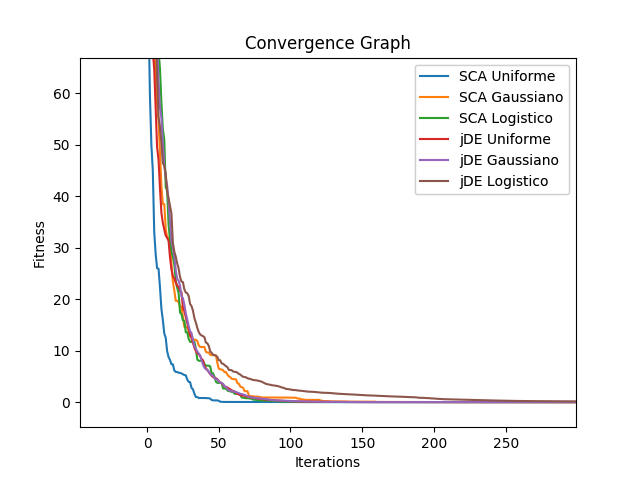
\includegraphics[width=0.49\linewidth]{figuras/convSphere.png}
    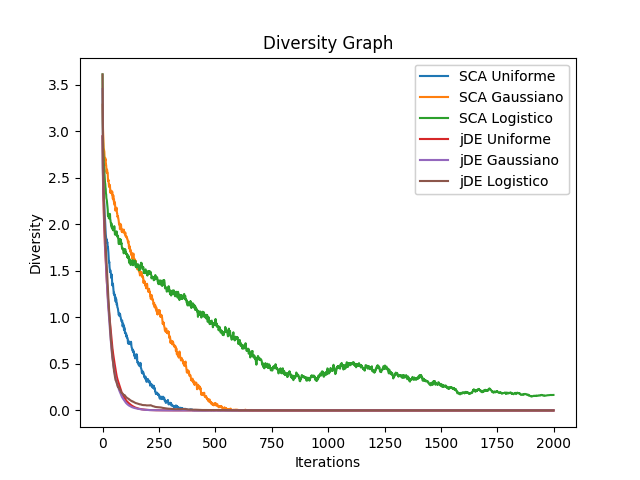
\includegraphics[width=0.49\linewidth]{figuras/divSphere.png}
    \captionof{figure}{Gráfico de Convergência (esquerda) e Gráfico de Diversidade (direita) dos Algoritmos para a Função Sphere}
    \label{fig:grafSphere}
    \source{Própria autora.}
}


{
    \centering
    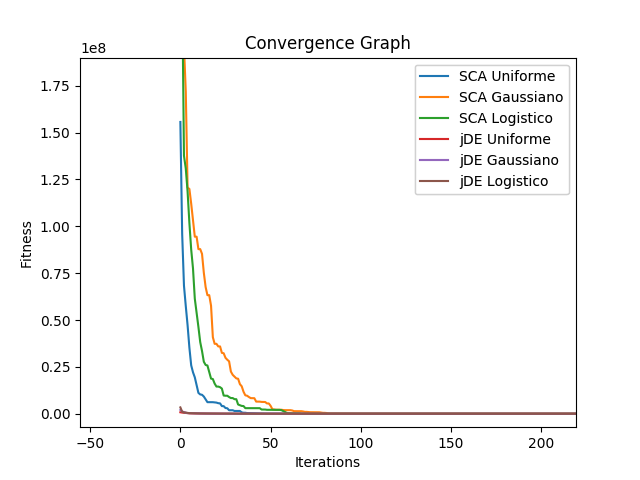
\includegraphics[width=0.49\linewidth]{figuras/convRosenbrock.png}
    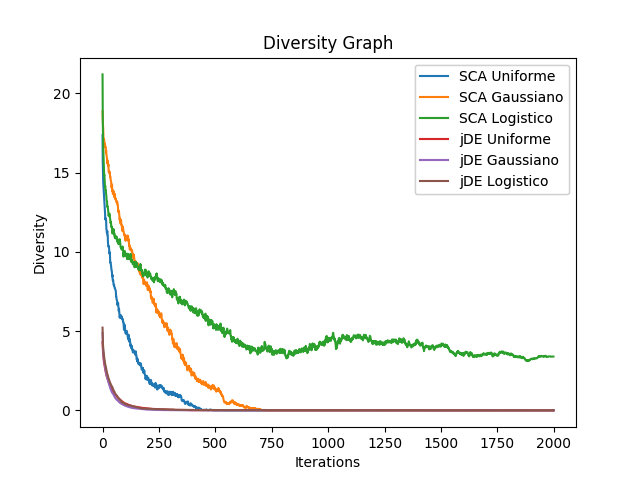
\includegraphics[width=0.49\linewidth]{figuras/divRosenbrock.png}
    \captionof{figure}{Gráfico de Convergência (esquerda) e Gráfico de Diversidade (direita) dos Algoritmos para a Função Rosenbrock}
    \label{fig:grafRosenbrock}
    \source{Própria autora.}
}

{
    \centering
    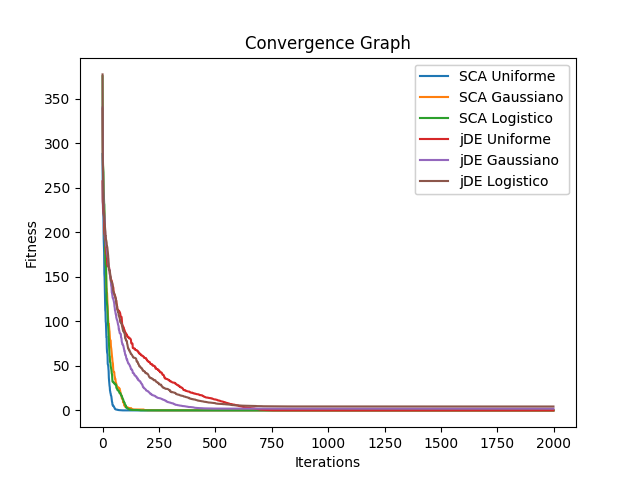
\includegraphics[width=0.49\linewidth]{figuras/convRastrigin.png}
    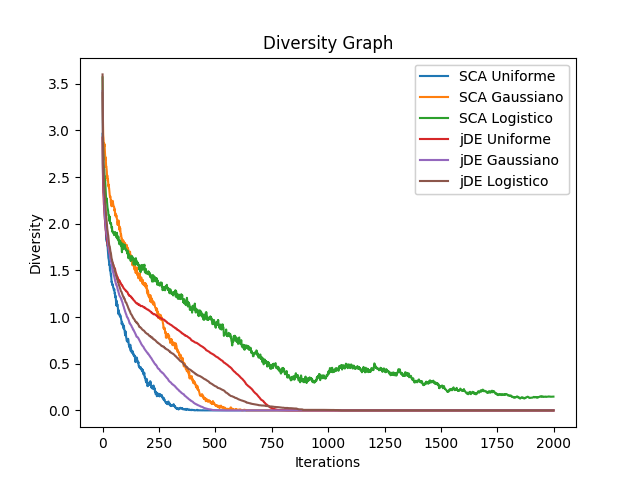
\includegraphics[width=0.49\linewidth]{figuras/divRastrigin.png}
    \captionof{figure}{Gráfico de Convergência (esquerda) e Gráfico de Diversidade (direita) dos Algoritmos para a Função Rastrigin}
    \label{fig:grafRastrigin}
    \source{Própria autora.}
}

{
    \centering
    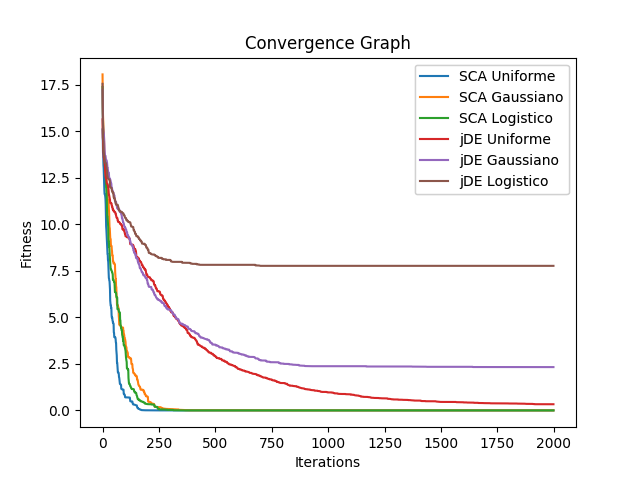
\includegraphics[width=0.49\linewidth]{figuras/convSchaffer.png}
    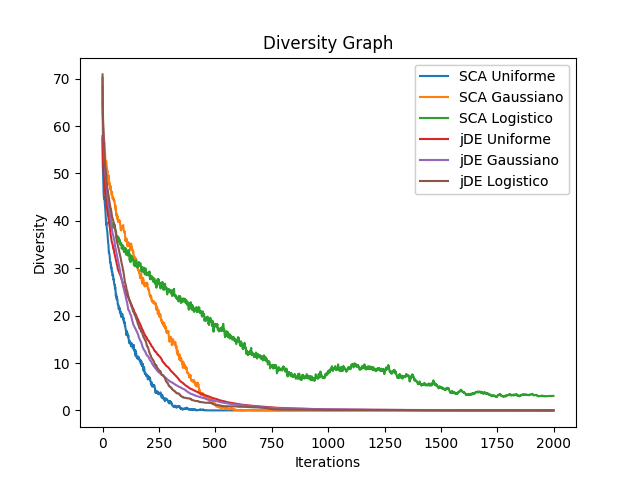
\includegraphics[width=0.49\linewidth]{figuras/divSchaffer.png}
    \captionof{figure}{Gráfico de Convergência (esquerda) e Gráfico de Diversidade (direita) dos Algoritmos para a Função Schaffer}
    \label{fig:grafSchaffer}
    \source{Própria autora.}
}

Além disso, também pode-se perceber a partir dos gráficos, que a diversidade dos algoritmos na maioria dos casos se encontra baixa - após algumas iterações, a diversidade chega a zero. A única exceção é o algoritmo SCA Logístico, que apresenta um comportamento diferente das outras meta-heurísticas, mantendo a diversidade mais alta durante o processo e decrescendo a curva de forma mais lenta.

{
    \centering
    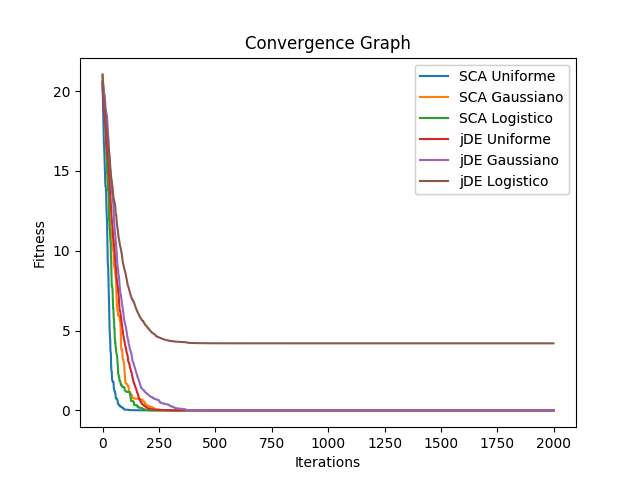
\includegraphics[width=0.49\linewidth]{figuras/convAckley.png}
    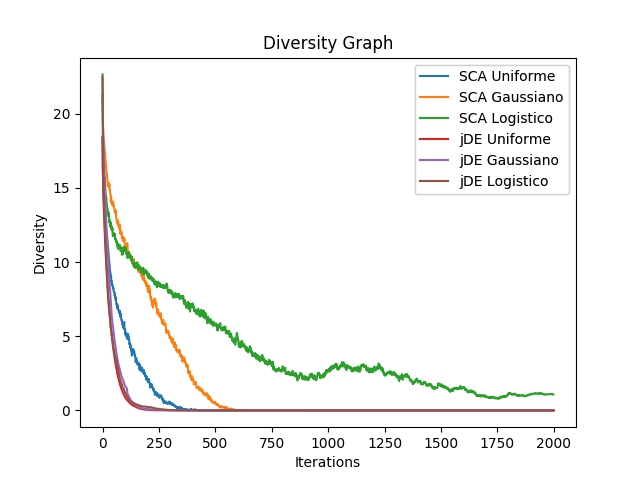
\includegraphics[width=0.49\linewidth]{figuras/divAckley.png}
    \captionof{figure}{Gráfico de Convergência (esquerda) e Gráfico de Diversidade (direita) dos Algoritmos para a Função Ackley}
    \label{fig:grafAckley}
    \source{Própria autora.}
}

{
    \centering
    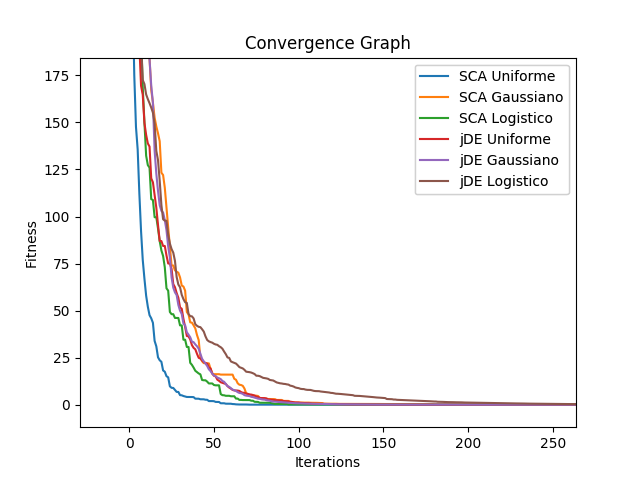
\includegraphics[width=0.49\linewidth]{figuras/convGriewank.png}
    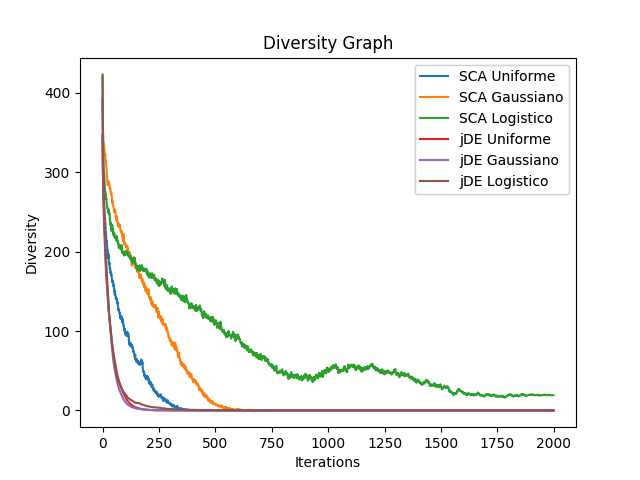
\includegraphics[width=0.49\linewidth]{figuras/divGriewank.png}
    \captionof{figure}{Gráfico de Convergência (esquerda) e Gráfico de Diversidade (direita) dos Algoritmos para a Função Griewank}
    \label{fig:grafGriewank}
    \source{Própria autora.}
}

{
    \centering
    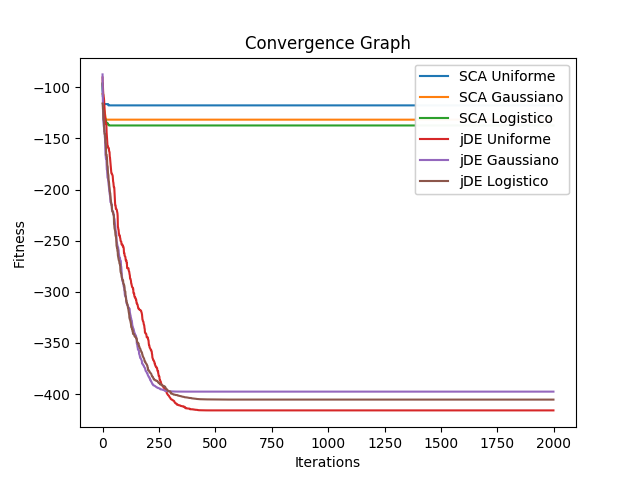
\includegraphics[width=0.49\linewidth]{figuras/convSchwefel.png}
    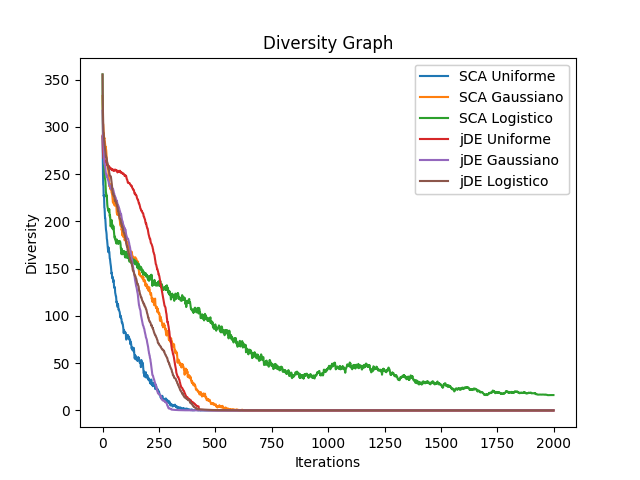
\includegraphics[width=0.49\linewidth]{figuras/divSchwefel.png}
    \captionof{figure}{Gráfico de Convergência (esquerda) e Gráfico de Diversidade (direita) dos Algoritmos para a Função Schwefel}
    \label{fig:grafSchwefel}
    \source{Própria autora.}
}

{
    \centering
    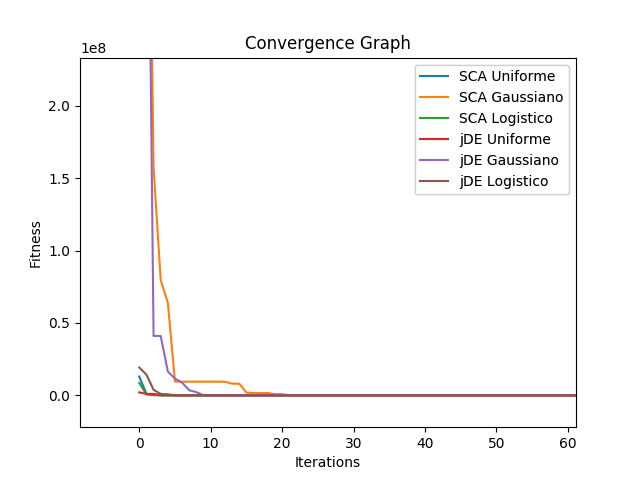
\includegraphics[width=0.49\linewidth]{figuras/convZakharov.png}
    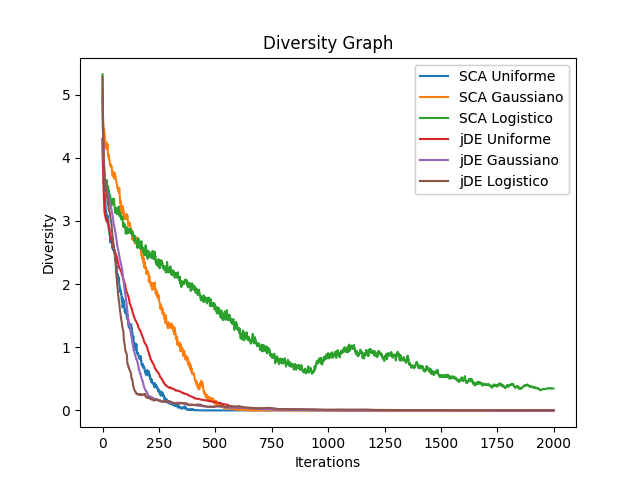
\includegraphics[width=0.49\linewidth]{figuras/divZakharov.png}
    \captionof{figure}{Gráfico de Convergência (esquerda) e Gráfico de Diversidade (direita) dos Algoritmos para a Função Zakharov}
    \label{fig:grafZakharov}
    \source{Própria autora.}
}


\section{Experimentos com PSP}
\label{sec:expPSP}

%Na primeira parte de desenvolvimento deste trabalho foram realizados experimentos que envolviam aplicar dois métodos de randomização em todas as partes dos algoritmos (jDE e SCA) que necessitam de aleatoriedade. Os métodos de randomização utilizados foram o mapa caótico Logístico e a distribuição Gaussiana, escolhidos devido ao fato de serem o mapa caótico e a distribuição mais populares, como visto no mapeamento sistemático da literatura. Esses algoritmos adaptados, foram então aplicados a um conjunto contendo oito funções \textit{benchmark}, e foram então comparados entre si e também com a versão original dos algoritmos, que utilizam a distribuição Uniforme. A comparação foi realizada através do cálculo da média e desvio-padrão das execuções de cada algoritmo, além da análise dos gráficos de convergência e diversidade dos mesmos.

%Os resultados destes experimentos, apresentados previamente no TCC-1, mostraram que nenhuma das versões adaptadas dos algoritmos se mostrou estatisticamente superior ao algoritmos originais. Sendo assim, como experimentos iniciais nesta seção, serão apresentadas as mesmas adaptações descritas no parágrafo anterior, mas aplicadas diretamente no problema de Predição da Estrutura de Proteínas. Esses experimentos possuem apenas o objetivo de verificar se o comportamento mostrado pelos algoritmos nos testes do TCC-1 se mantém o mesmo em um problema do mundo real.

Dois experimentos distintos foram executados aplicando algoritmos no problema da Predição da Estrutura de Proteínas. O primeiro experimento envolve utilizar as mesmas adaptações usadas nos testes com \textit{benchmarks}, e possui o objetivo de verificar se o comportamento mostrado pelos algoritmos nas funções de teste se mantém o mesmo em um problema do mundo real, como o PSP. Já o segundo experimento envolve utilizar a aplicação descrita na seção \ref{sec:apPontosEsp}, com o objetivo de verificar se a abordagem desenvolvida, usando uma aplicação em pontos específicos do algoritmo (parâmetros r2 e r3), com uma distribuição Gaussiana com desvio-padrão adaptado e uma técnica de \textit{crowding}, possui um desempenho superior quando comparado com o algoritmo SCA original.

\subsection{Configurações}
\label{sec:config}

As configurações utilizadas nos experimentos, foram as seguintes:

\begin{itemize}
    \item Tamanho da população: 30;
    \item Gerações: 10000;
    \item Execuções: 30;
\end{itemize}

Além destas, para a segunda parte dos experimentos, tem-se os parâmetros da técnica de \textit{crowding}: o fator de \textit{crowding} foi definido como 3; e a porcentagem da população que é atualizada, ou seja, a quantidade de filhos ou \textit{offspring} gerada é igual a 80\% da população original.

\subsection{Sequências de Proteínas}

O conjunto de proteínas utilizadas envolvem quatro sequências \textit{benchmark} de proteínas, utilizadas através do modelo \textit{off-lattice} 2D-AB. As sequências, assim como o número de aminoácidos presentes nelas, ou seja, a quantidade de dimensões que a instância do problema possui, são apresentadas na tabela \ref{tab:sequencias}.


\begin{table}[!htpb]
    \centering
    \begin{tabularx}{\textwidth}{c|X} % <-- Alignments: 1st column left, 2nd middle and 3rd right, with vertical lines in between
    
      \textbf{N} & \textbf{Sequência}\\
      \hline
      13 & ABBABBABABBAB\\
      \hline
      21 & BABABBABABBABBABABBAB\\
      \hline
      34 & ABBABBABABBABBABABBABABBABBABABBAB\\
      \hline
      55 & BABABBABABBABBABABBABABBABBABABBAB \newline BABABBABABBABBABABBAB\\
    \end{tabularx}
    \caption{Conjunto de Sequências Proteicas Usadas}
    \label{tab:sequencias}
\end{table}

\subsection{Resultados e Análises da Aplicação em Todos os Pontos}

Os resultados do primeiro experimento com PSP, com aplicação em todos os pontos de aleatoriedade do algoritmo, podem ser observados na tabela \ref{tab:resultadosIniciais}, estruturada da mesma forma que a tabela de resultados anterior: o primeiro valor encontrado é a média das execuções e o segundo valor é o desvio-padrão. Cada linha da tabela representa uma sequência de proteínas, e cada coluna da tabela representa uma das distribuições utilizadas, sendo que para cada uma destas, tem-se a separação entre os dois algoritmos, jDE e SCA. A última linha da tabela representa o somatório de vezes que determinado algoritmo foi estatisticamente o melhor para certa função, sendo que os melhores resultados foram determinados a partir dos testes estatísticos de Kruskall-Vallis e de Dunn.

\begin{center}
\renewcommand{\arraystretch}{2.0}
{\scriptsize
\setlength\LTleft{-10pt}
%\setlength\LTright{-40pt}
\begin{longtable}{c|c c c c c c}
\\ %\hline
\multirow{2}{*}{Função} & \multicolumn{2}{c}{Uniforme} & \multicolumn{2}{c}{Gaussiana} & 
\multicolumn{2}{c}{Logístico} \\
& jDE & SCA & jDE & SCA & jDE & SCA\\
\hline \endhead
$F_{13}$ & \makecell{{\bf-1,9189e+00 $\pm$}\\{\bf3,6629e-01}} 
      & \makecell{{-0,5874e+00 $\pm$} \\ {0,0921e+00}} 
      & \makecell{{\bf-1,7748e+00 $\pm$} \\ {\bf3,9848e-01}}
      & \makecell{{-0,5902e+00  $\pm$} \\ {0,0612e+00} }
      & \makecell{{-1,4509e+00 $\pm$ }\\ {7,0879e-01}} 
      & \makecell{{-0,7968e+00 $\pm$} \\ {0,1745e+00}}\\ %\hline

$F_{21}$  & \makecell{{\bf-4,0581e+00 $\pm$}\\{\bf3,8556e-01}}
      & \makecell{{-1,0345e+00 $\pm$} \\ {0,1064e+00}} 
      & \makecell{{\bf-3,5875e+00 $\pm$} \\ {\bf7,5970e-01}}
      & \makecell{{-1,0738e+00 $\pm$} \\ {0,0967e+00} }
      & \makecell{{-2,9871e+00 $\pm$} \\ {1,2664e+00}}
      & \makecell{{-1,2132e+00 $\pm$ }\\ {0,1360e+00}} \\

$F_{34}$  & \makecell{{\bf-6,6902e+00$\pm$}\\{\bf8,9389e-01}} 
      & \makecell{{-0,9526e+00 $\pm$} \\ {0,2652e+00}} 
      & \makecell{{\bf-5,7044e+00 $\pm$} \\ {\bf1,3987e+00}}
      & \makecell{{-1,0135e+00 $\pm$} \\ {0,2500e+00} }
      & \makecell{{-4,8845e+00 $\pm$} \\ {1,8677e+00}}
      & \makecell{{-1,2386e+00 $\pm$ }\\ {0,2906e+00}} \\
        
$F_{55}$ & \makecell{{\bf-9,6476e+00 $\pm$} \\ {\bf1,3193e+00}} 
      & \makecell{{-1,2564e+00 $\pm$} \\ {0,1734e+00}} 
      & \makecell{{2,5832e+01 $\pm$} \\ {1,8098e+02} }
      & \makecell{{-1,2265e+00 $\pm$} \\ {0,1684e+00} }
      & \makecell{{2,6790e+01  $\pm$} \\ {1,8101e+02}}
      & \makecell{{-1,4580e+00 $\pm$ }\\ {0,3562e+00}} \\
    
    \hline
\makecell{Destaques} & 4  & 0  & 3 & 0  &
0  & 0 \\

\caption{Resultados do Primeiro Experimento com PSP}
\label{tab:resultadosIniciais}
\end{longtable}
}
%\footnotesize{Fonte: autoria própria.}
\end{center}

Através dos destaques, pode-se observar que o algoritmo jDE com distribuição Uniforme teve o melhor desempenho dentre todos, possuindo o melhor resultado em todas as quatro instâncias do problema. Em seguida, tem-se o jDE com distribuição Gaussiana, que mostrou resultados equivalentes ao do jDE Uniforme em três das instâncias. E por fim, todos os outros algoritmos apresentaram um desempenho ruim, não alcançando os melhores resultados em nenhuma das instâncias do problema. Além disso, pode-se perceber como as versões do algoritmo jDE, de modo geral, obtiveram resultados superiores as versões do algoritmo SCA, mostrando que entre os dois, o jDE se apresenta como a melhor escolha para um problema do mundo real complexo como o PSP.

Em relação às diferentes distribuições utilizadas, tem-se que para o algoritmo jDE, a distribuição Uniforme continuou sendo a melhor escolha, apresentando a maior consistência em seus resultados. A distribuição Gaussiana mostrou desempenho similar nas primeiras instâncias do problema, entretanto, na instância com 55 dimensões, uma das suas 30 execuções teve dificuldade para convergir, ficando presa em um ótimo local - isso fez com que seu resultado para essa sequência decaísse bastante. O mapa caótico Logístico teve o mesmo problema na instância de 55 dimensões, além de mostrar resultados piores em todas as outras instâncias, sendo a pior escolha de método de randomização para ser utilizado no algoritmo jDE com esse tipo de abordagem de adaptação. Essa conclusão foi inesperada, visto que na literatura esse mapa caótico tem mostrado bons resultados em outros problemas e algoritmos.

Para o algoritmo SCA, tem-se que todas as suas versões apresentaram resultados bem próximos, entretanto, por mais que a diferença tenha sido pequena, os testes estatísticos mostraram que a versão que utiliza o mapa caótico Logístico apresentou resultados superiores. Sendo assim, a melhor escolha de método de randomização para o algoritmo SCA com a adaptação em todos os pontos de aleatoriedade, seria o mapa Logístico. Em sequência, pelo desempenho, tem-se a distribuição Gaussiana e por fim, a distribuição Uniforme. Essa conclusão foi exatamente o oposto do que foi visto no algoritmo jDE, e nos experimentos realizados anteriormente nas funções \textit{benchmark}. Isso comprova que o tipo de método de randomização que deve ser utilizado, ou seja, que trará um melhor desempenho, está diretamente ligado ao algoritmo usado e ao problema na qual o mesmo será aplicado. Sendo assim, a escolha para método de randomização varia dependendo do problema, do algoritmo e também do tipo de abordagem utilizada, ou seja, em que pontos do algoritmo que esse método de randomização é aplicado.

% f13 - sca log
% f21 - sca log
% f34 - sca log e sca gauss
% f55 - sca log, sca gauss e sca uni

Os gráficos de convergência e de diversidade dos algoritmos para cada uma das quatro sequências proteicas podem ser visualizados nas figuras \ref{fig:grafF13ExpIni} até \ref{fig:grafF55ExpIni}. 

{
    \centering
    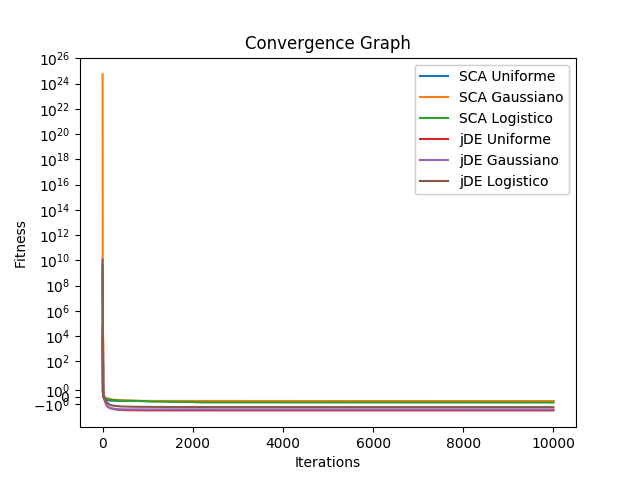
\includegraphics[width=0.49\linewidth]{figuras/convF13.png}
    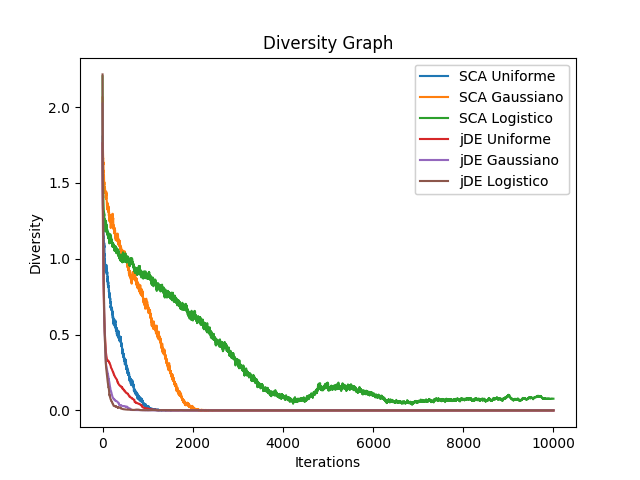
\includegraphics[width=0.49\linewidth]{figuras/divF13.png}
    \captionof{figure}{Gráfico de Convergência dos Algoritmos (esquerda) e Gráfico de Diversidade dos Algoritmos (direita) para a Sequência F13}
    \label{fig:grafF13ExpIni}
    \source{Própria autora.}
}

{
    \centering
    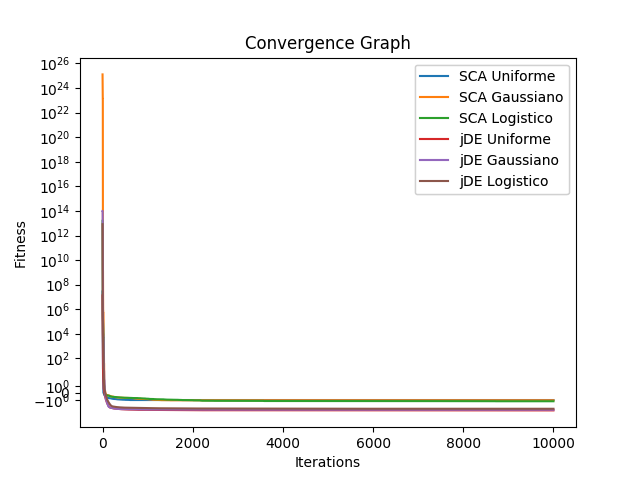
\includegraphics[width=0.49\linewidth]{figuras/convF21.png}
    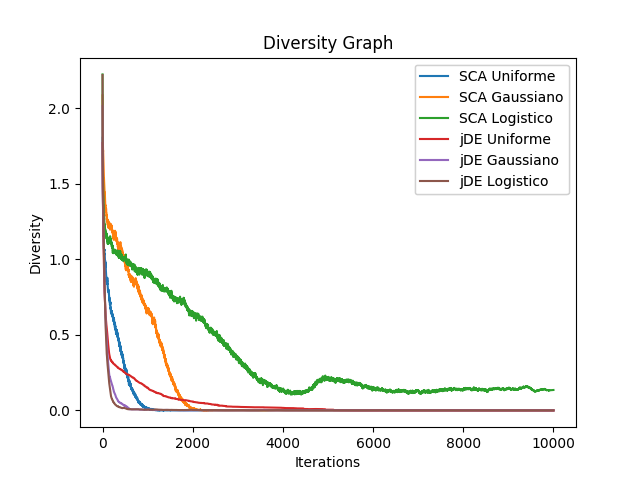
\includegraphics[width=0.49\linewidth]{figuras/divF21.png}
    \captionof{figure}{Gráfico de Convergência dos Algoritmos (esquerda) e Gráfico de Diversidade dos Algoritmos (direita) para a Sequência F21}
    \label{fig:grafF21ExpIni}
    \source{Própria autora.}
}

{
    \centering
    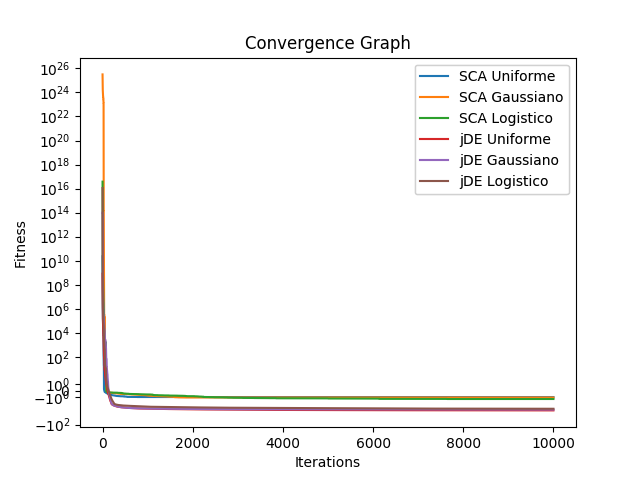
\includegraphics[width=0.49\linewidth]{figuras/convF34.png}
    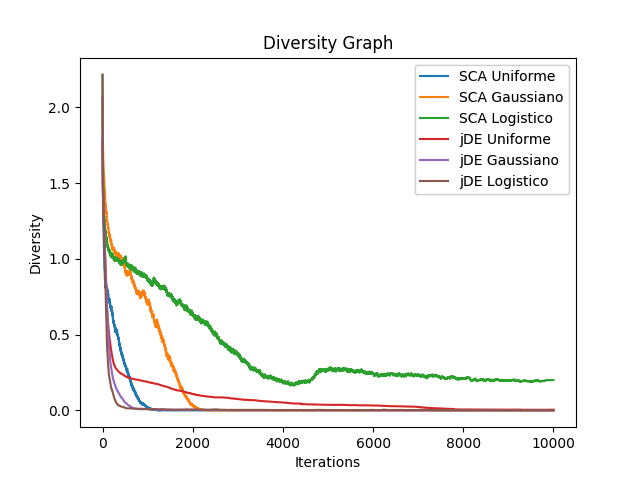
\includegraphics[width=0.49\linewidth]{figuras/divF34.png}
    \captionof{figure}{Gráfico de Convergência dos Algoritmos (esquerda) e Gráfico de Diversidade dos Algoritmos (direita) para a Sequência F34}
    \label{fig:grafF34ExpIni}
    \source{Própria autora.}
}

{
    \centering
    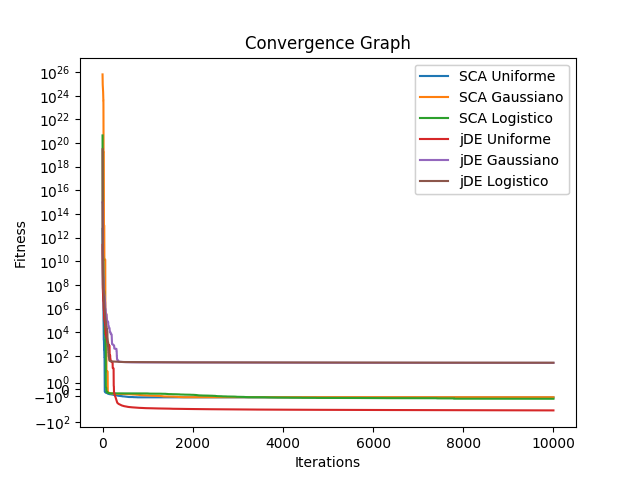
\includegraphics[width=0.49\linewidth]{figuras/convF55.png}
    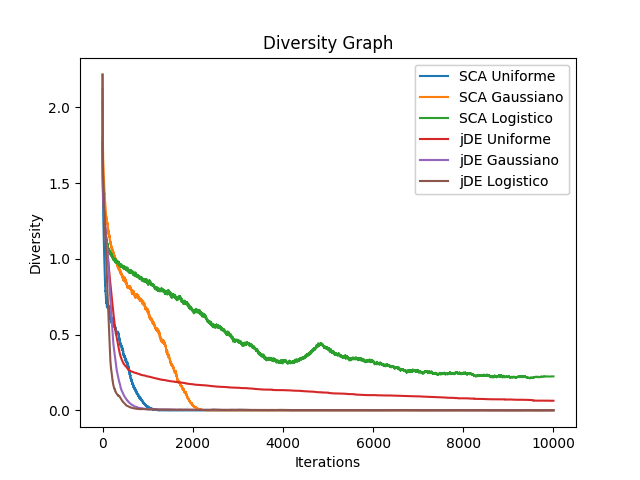
\includegraphics[width=0.49\linewidth]{figuras/divF55.png}
    \captionof{figure}{Gráfico de Convergência dos Algoritmos (esquerda) e Gráfico de Diversidade dos Algoritmos (direita) para a Sequência F55}
    \label{fig:grafF55ExpIni}
    \source{Própria autora.}
}

Analisando os gráficos, pode-se observar que a convergência dos algoritmos foi extremamente rápida e abrupta para todas as instâncias do problema. Em média, nas primeiras 30 gerações do processo de otimização, os algoritmos já convergem para um ótimo, e aproveitam o restante das gerações para refinar as soluções a partir deste ótimo encontrado. Além disso, pode-se perceber que a diversidade dos algoritmos teve um comportamento similar para todas as instâncias do problema PSP e, com exceção do SCA com mapa Logístico, os algoritmos perderam a diversidade, chegando a zero, após cerca de 2000 a 4000 gerações.


\subsection{Resultados e Análises da Aplicação em Pontos Específicos}

%Como experimentos finais deste trabalho, foram realizados testes aplicando a versão adaptada do SCA, implementada de acordo com a seção \ref{sec:proposta}, no problema de Predição da Estrutura de Proteínas. A versão adaptada foi comparada com a versão original (padrão) do algoritmo SCA, usando como base a média e desvio-padrão das execuções de cada algoritmo, além da análise dos gráficos de convergência e diversidade.

%As configurações utilizadas para estes experimentos são as mesmas que se encontram na seção \ref{sec:config}, com adição dos parâmetros da técnica de \textit{crowding}: o fator de \textit{crowding} foi definido como 3; e a porcentagem da população que é atualizada, ou seja, a quantidade de filhos ou \textit{offspring} gerada é igual a 80\% da população original. Além disso, as sequências de proteínas aplicadas no algoritmo são as mesmas da tabela \ref{tab:sequencias}.

Os resultados dos experimentos executados, a partir da abordagem apresentada em \ref{sec:apPontosEsp}, podem ser observados na tabela \ref{tab:resultadosFinaisExp}, estruturada da mesma forma que as tabelas de resultados anteriores.

\begin{center}
\renewcommand{\arraystretch}{2.0}
{\footnotesize
\begin{longtable}{c|c c}
\\ %\hline
Função & SCA Padrão & SCA Adaptado
\\
\hline \endhead
$F_{13}$ & \makecell{{-0,5874e+00 $\pm$} \\ {0,0921e+00}} 
      & \makecell{{\bf-1,9444e+00 $\pm$} \\ {\bf0,3340e+00}} \\ 

$F_{21}$  & \makecell{{-1,0345e+00 $\pm$} \\ {0,1064e+00}} 
      & \makecell{{\bf-2,5988e+00 $\pm$} \\ {\bf0,4972e+00}}  \\

$F_{34}$ & \makecell{{-0,9526e+00 $\pm$} \\ {0,2652e+00}} 
      & \makecell{{\bf-2,9768e+00 $\pm$} \\ {\bf0,6780e+00}}  \\
        
$F_{55}$ & \makecell{{-1,2564e+00 $\pm$} \\ {0,1734e+00}} 
      & \makecell{{\bf-3,3634e+00 $\pm$} \\ {\bf1,0257e+00}}  \\
    
    \hline
\makecell{Destaques} & 0  & 4  \\

\caption{Resultados do Segundo Experimento com PSP}
\label{tab:resultadosFinaisExp}
\end{longtable}
}
%\footnotesize{Fonte: autoria própria.}
\end{center}

Através dos destaques, pode-se perceber que para todas as instâncias do problema PSP a versão adaptada do algoritmo SCA obteve um desempenho superior ao do algoritmo original. Isso nos mostra como a adaptação realizada foi eficaz e comprova que, assim como visto nos experimentos iniciais, em certos casos a utilização de um método de randomização diferente do Uniforme é benéfica para o algoritmo. Com isso, pode-se concluir que não só o método de randomização usado para gerar números aleatórios afeta diretamente os resultados e o desempenho dos algoritmos estocásticos, como também que deve ser feita uma escolha de qual método utilizar. Ou seja, o método de randomização acaba se tornando um outro parâmetro das meta-heurísticas, que além de ser extremamente importante, dever ser escolhido com cuidado, levando em consideração vários aspectos como: o algoritmo que está sendo usado; o problema ao qual o algoritmo está tentando solucionar; e em que partes do algoritmo este método foi aplicado.

Além disso, fica claro que a abordagem utilizada nessa adaptação, fazendo a troca do método de randomização em pontos específicos do algoritmo, trouxe benefícios, como a melhora dos resultados. Isso explica o porquê dessa abordagem ter sido a mais utilizada nos artigos encontrados no mapeamento sistemático da literatura. Entretanto, é válido apontar que essa abordagem tem suas desvantagens, como por exemplo a dificuldade de implementação. Para desenvolvê-la, é necessário compreender a fundo como o algoritmo em questão funciona e como é seu comportamento ao longo das gerações do processo de otimização. Além disso, é preciso identificar os pontos de interesse da meta-heurística, os parâmetros que mais afetam seu desempenho. Esse processo pode ser em muitos casos demorado e trabalhoso, enquanto a abordagem apresentada nos experimentos iniciais, trocando o método utilizado em todos os pontos de aleatoriedade do algoritmo, é muito mais simples.

Os gráficos de convergência e de diversidade dos algoritmos SCA original e SCA adaptado para cada uma das quatro sequências proteicas podem ser visualizados nas figuras \ref{fig:grafF13ExpFinal} até \ref{fig:grafF55ExpFinal}.

{
    \centering
    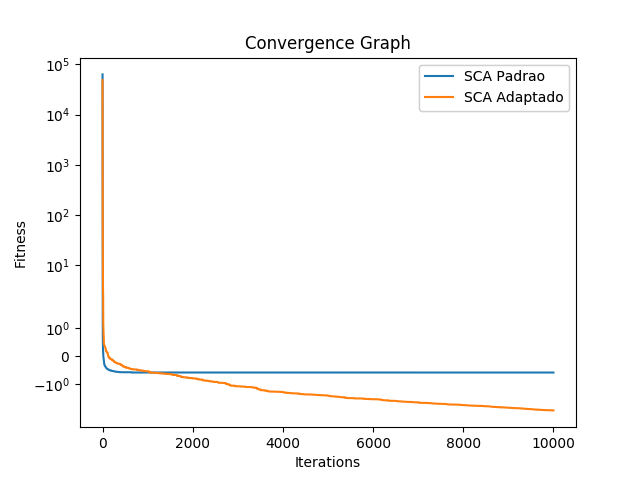
\includegraphics[width=0.49\linewidth]{figuras/convF13_F.png}
    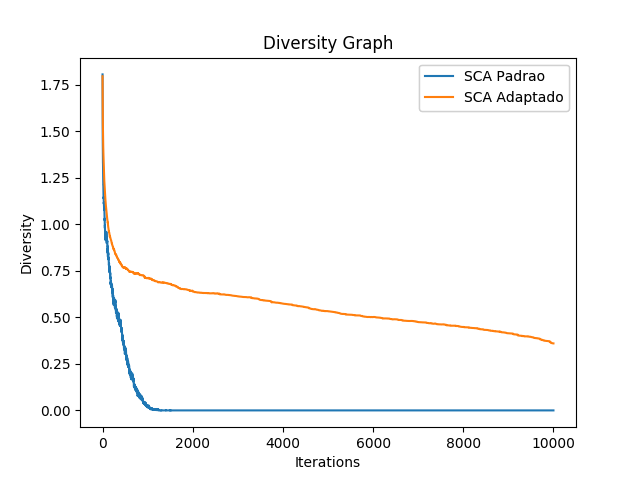
\includegraphics[width=0.49\linewidth]{figuras/divF13_F.png}
    \captionof{figure}{Gráfico de Convergência (esquerda) e Gráfico de Diversidade (direita) dos Dois Algoritmos para a Sequência F13}
    \label{fig:grafF13ExpFinal}
    \source{Própria autora.}
}

{
    \centering
    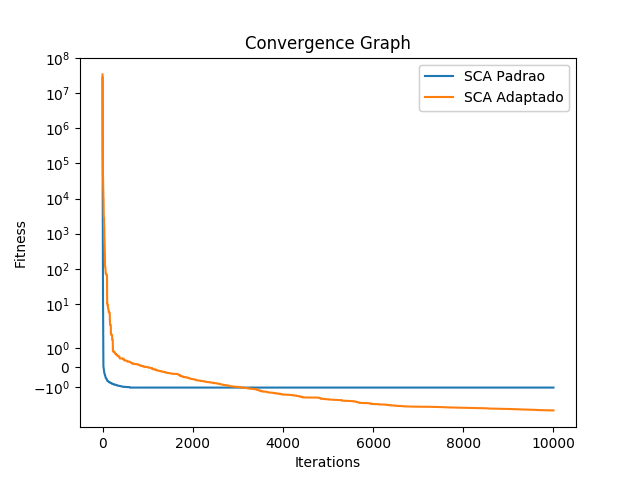
\includegraphics[width=0.49\linewidth]{figuras/convF21_F.png}
    \includegraphics[width=0.49\linewidth]{figuras/divF21_F.png}
    \captionof{figure}{Gráfico de Convergência dos Algoritmos (esquerda) e Gráfico de Diversidade dos Algoritmos (direita) para a Sequência F21}
    \label{fig:grafF21ExpFinal}
    \source{Própria autora.}
}

{
    \centering
    \includegraphics[width=0.49\linewidth]{figuras/convF34_F.png}
    \includegraphics[width=0.49\linewidth]{figuras/divF34_F.png}
    \captionof{figure}{Gráfico de Convergência (esquerda) e Gráfico de Diversidade (direita) dos Dois Algoritmos para a Sequência F34}
    \label{fig:grafF34ExpFinal}
    \source{Própria autora.}
}

{
    \centering
    \includegraphics[width=0.49\linewidth]{figuras/convF55_F.png}
    \includegraphics[width=0.49\linewidth]{figuras/divF55_F.png}
    \captionof{figure}{Gráfico de Convergência (esquerda) e Gráfico de Diversidade (direita) dos Dois Algoritmos para a Sequência F55}
    \label{fig:grafF55ExpFinal}
    \source{Própria autora.}
}

Analisando os gráficos, pode-se observar que a convergência do algoritmo SCA padrão foi rápida e abrupta para todas as instâncias do problema e, que em todos os casos, o algoritmo ficou preso em um ótimo local pela maioria das iterações. Já o SCA adaptado mostrou uma convergência rápida apenas nas duas primeiras funções, F13 e F21, enquanto que nas sequências F34 e F55, sua convergência foi mais lenta. Um ponto a se destacar é que o SCA adaptado não ficou preso permanentemente em ótimos locais - pode-se visualizar que sua curva de convergência continua a decrescer até o final das gerações, mesmo na sequência F55, onde pode-se observar que o algoritmo conseguiu escapar de um forte atrator local.

Além disso, pode-se perceber que a diversidade do algoritmo original chega a zero após algumas iterações, enquanto o SCA adaptado apresenta uma diversidade maior durante o processo, decrescendo de forma lenta. Esse comportamento é um resultado conjunto entre a utilização da distribuição Gaussiana com a técnica de \textit{crowding}, responsável por desacelerar a perda de diversidade.

Outro ponto importante para se analisar é como o desempenho do SCA adaptado se compara com o desempenho de outros algoritmos da literatura para o problema PSP 2-D AB, além do SCA original. Para isso, apresenta-se para comparação três algoritmos: \textit{Improved PSO Algorithm} (PSO) \cite{xiaolong}; \textit{Improved Energy Landscape Paving} (ELP+) \cite{liu}; e \textit{Conformational Space Annealing} (CSA) \cite{kim}.


\begin{center}
\renewcommand{\arraystretch}{2.0}
{\footnotesize
\begin{longtable}{c|c c c c}
\\ %\hline
Função & PSO & ELP+ & CSA & SCA Adaptado
\\
\hline \endhead
$F_{13}$ & \makecell{{-3,2941}} 
      & \makecell{{-3,2941}}
      & \makecell{{-3,2941}}
      & \makecell{{-3,1766}}\\ 

$F_{21}$  & \makecell{{-6,1977}} 
      & \makecell{{-6,1980}}
      & \makecell{{-6,1980}}
      & \makecell{{-3,5372}}\\

$F_{34}$ & \makecell{{-10,7036}} 
      & \makecell{{-10,7453}}
      & \makecell{{-10,8060}}
      & \makecell{{-4,1649}}\\
        
$F_{55}$ & \makecell{{-18,4236}} 
      & \makecell{{-18,9301}}
      & \makecell{{-18,9110}}
      & \makecell{{-7,1168}}\\
\caption{Resultados dos Algoritmos para Comparação}
\label{tab:resultadosComparacoes}
\end{longtable}
}
%\footnotesize{Fonte: autoria própria.}
\end{center}

Como pode-se visualizar na tabela \ref{tab:resultadosComparacoes}, tem-se as energias mínimas (melhores resultados de um conjunto de execuções) que foram encontradas pelos algoritmos para cada uma das sequências de proteínas. Pode-se perceber, através destes valores absolutos, que o algoritmo SCA adaptado possui um desempenho próximo dos outros apenas na primeira sequência de proteína, com 13 aminoácidos. Nos outros casos, seus resultados são inferiores em comparação com esses três algoritmos da literatura. Entretanto, para realizar uma comparação justa, deve-se levar em consideração o esforço computacional usado pelos diferentes algoritmos: os estudos que apresentaram o ELP+ e CSA não deixaram explícito o número de avaliações de função ou iterações usadas. Já de acordo com \cite{xiaolong}, o PSO utilizou um total de 20 mil iterações, enquanto o SCA adaptado, algoritmo apresentado aqui, utilizou 10 mil iterações no total. Dessa forma, talvez o SCA adaptado apresentasse melhores resultados com mais iterações - mas essa hipótese não foi testada nos experimentos por questão de tempo de execução. O algoritmo, com os parâmetros citados nas configurações, já demorava um tempo considerável para realizar suas 30 execuções, visto que foi implementado de forma sequencial, e não paralela.

%O que mais?